% Authoritative arXiv source. Compile with pdfLaTeX; no external assets are used.
\pdfoutput=1
\documentclass[11pt,letterpaper]{article}
\usepackage[T1]{fontenc}
\usepackage[utf8]{inputenc}
\usepackage{lmodern}
\usepackage{microtype}
\usepackage{amsmath,amssymb,amsthm,mathtools}
\usepackage[margin=1in]{geometry}
\usepackage{booktabs,array,tabularx}
\usepackage[dvipsnames]{xcolor}
\usepackage{tikz}
\usetikzlibrary{arrows.meta,positioning}
\usepackage{hyperref}
\IfFileExists{cleveref.sty}{
  \usepackage[nameinlink,capitalise,noabbrev]{cleveref}
}{
  \newcommand{\cref}[1]{\ref{#1}}
  \let\Cref\cref
}
\urlstyle{same}
\hypersetup{
  pdftitle={Almost-Everywhere Near-Cubic Wire Lower Bounds for SYM o THR
and THR o THR},
  pdfauthor={Dev Nag},
  colorlinks=true,
  linkcolor={blue},
  filecolor={Maroon},
  citecolor={Blue},
  urlcolor={blue},
  pdfcreator={LaTeX}}

\newtheorem{theorem}{Theorem}[section]
\newtheorem{lemma}[theorem]{Lemma}
\newtheorem{proposition}[theorem]{Proposition}
\newtheorem{corollary}[theorem]{Corollary}
\newtheorem{fact}[theorem]{Fact}
\theoremstyle{definition}
\newtheorem{definition}[theorem]{Definition}
\theoremstyle{remark}
\newtheorem{remark}[theorem]{Remark}

\newcommand{\CAPP}{\textsc{CAPP}}
\newcommand{\ANDfour}{\textsc{AND}_{\le 4}}
\newcommand{\Ftwo}{\mathbb F_2}
\newcommand{\poly}{\operatorname{poly}}
\newcommand{\polylog}{\operatorname{polylog}}
\newcommand{\Eclass}{\mathrm E^{\mathrm{NP}}}
\newcommand{\SYMTHR}{\mathrm{SYM}\circ\mathrm{THR}}
\newcommand{\THRTHR}{\mathrm{THR}\circ\mathrm{THR}}
\setcounter{tocdepth}{2}
\setcounter{secnumdepth}{3}
\setlength{\emergencystretch}{3em}

\title{Almost-Everywhere Near-Cubic Wire Lower Bounds for
\(\SYMTHR\) and \(\THRTHR\)}
\author{Dev Nag\\
CtrlStack, Inc.\\
\texttt{devnag@gmail.com}\\
\href{https://orcid.org/0009-0006-7304-8082}{\nolinkurl{https://orcid.org/0009-0006-7304-8082}}}
\date{August 17, 2026}

\begin{document}
\maketitle
\begin{abstract}
Kane and Williams proved average-case wire lower bounds at the
\(n^{5/2}/\polylog n\) scale for an explicit function against depth-two
linear-threshold circuits. We prove an almost-everywhere near-cubic wire
lower bound for a language in \(\Eclass\). For every fixed \(c>0\), there is
one language \(F_c\) and positive constants \(b_{\mathrm S,c}\) and
\(b_{\mathrm T,c}\) such that, at every sufficiently large input length
\(n\), no \(\SYMTHR\) circuit with at most
\(b_{\mathrm S,c}n^3/\log^{10}n\) wires and no \(\THRTHR\) circuit with at
most \(b_{\mathrm T,c}n^3/\log^{12}n\) wires has agreement at least
\(1/2+n^{-c}\) with \((F_c)_n\). The same language works for both
classes, and the gates may have arbitrary real weights. At any fixed positive
advantage, the logarithmic denominators improve to \(\log^5n\) and
\(\log^9n\).

The algorithmic core is a deterministic circuit-acceptance-probability
algorithm that charges a restricted circuit by the number of input wires
touching the live variables, rather than by its number of bottom gates. Exact
residualization removes both constant-zero and constant-one bottom gates from
the algebraic population. Multiscale counting polynomials and exact signed
rectangular multiplication then give inverse-polynomially accurate analysis
with an arbitrary fixed polynomial saving. A componentwise
Chen--Lyu--Williams transfer, its XOR contrapositive, and an exact length
schedule yield the stated correlation lower bounds.
\end{abstract}

\medskip
\noindent\textbf{Keywords:} circuit lower bounds; threshold circuits; wire
complexity; circuit analysis; hardness amplification.

\tableofcontents

\section{Introduction}\label{sec:introduction}

\subsection{Result and contribution}\label{sec:result-contribution}

Wire complexity is the natural resource when a depth-two circuit may contain
many bottom gates with very small support. Gate-count arguments treat all
bottom gates alike; a wire bound must instead account for how often input
variables actually occur. The strongest previous average-case lower bound in
this unrestricted simple-edge setting is the
\(n^{5/2}/\polylog n\)-scale theorem of Kane and Williams. We raise the wire
exponent to \(3-o(1)\), at the cost of placing the hard language in
\(\Eclass\) rather than linear time.

More precisely, for every fixed \(c>0\), one language is hard at every
sufficiently large length against both \(\SYMTHR\) and \(\THRTHR\). Agreement
\(1/2+n^{-c}\) requires, respectively, more than a fixed positive multiple of
\(n^3/\log^{10}n\) and \(n^3/\log^{12}n\) wires. The circuit gates may have
arbitrary real weights, and there is no separate bound on the number or
support sizes of the bottom gates. \Cref{thm:main-inverse} gives the formal
statement.

The main algorithmic contribution is a deterministic
\emph{circuit-acceptance-probability problem} (\CAPP) algorithm for a
conjunction of at most four input circuits; we abbreviate this task by
\(\ANDfour\)-\CAPP. After keeping \(K=\Theta(\log n)\) variables live, the
algorithm charges only bottom supports that touch the live set. Exact
residualization removes both constant-zero and constant-one restricted gates.
The resulting polynomial degree depends on the square root of the touched
population, enabling the near-cubic wire cap. The supplier theorems
\cref{thm:supplier-inverse} and \cref{thm:supplier-fixed} may be of independent
algorithmic interest.

\subsection{Related work}\label{sec:related-work}

Threshold logic originates in the work of Muroga, Toda, and Takasu
\cite{MTT61}; standard background includes Muroga's monograph \cite{Mur71},
comparisons between majority and weighted threshold gates \cite{HG91,GHR92},
bounded-depth threshold circuits \cite{HMPST93}, and finite integer-weight
normalization \cite{Has94}. At depth two, relevant satisfiability and counting
algorithms include the sparse-wire regime \cite{IPS13}, dense special cases
\cite{AS15}, average-case analysis of small threshold circuits \cite{CSS18},
polynomial-representation methods \cite{ACW16}, Tamaki's subquadratic-gate
algorithm \cite{Tam16}, and Williams's satisfiability algorithm for
\(\mathrm{ACC}\circ\mathrm{THR}\) circuits \cite{Wil14}, the first contact of
the algorithmic method with unbounded-weight threshold gates. These
results provide context; the supplier proved here
does not use them as black boxes.

Wire lower bounds for threshold circuits begin with Impagliazzo, Paturi,
and Saks \cite{IPS97}: at depth \(d\), computing parity requires
\(n^{1+c^{-d}}\) wires for a fixed \(c>1\), and at depth two it requires
\(\Omega(n^{3/2})\) wires. The nearest wire theorem is due to Kane and
Williams \cite[Theorem 1.1]{KW16}. They proved that the linear-time
computable Andreev function \cite{And87} cannot have agreement
\(1/2+\varepsilon\) with a depth-two linear-threshold circuit using
\(o(\varepsilon^3n^{5/2}/\log^{7/2}n)\) wires, in their stated range
\(\varepsilon\gg\sqrt{\log n/n}\). At advantage \(\varepsilon=n^{-c}\)
with \(c>1/2\) that theorem is outside its stated range, and inside the
range its wire scale decays with \(\varepsilon^3\); the
inverse-polynomial-advantage regime of \cref{thm:main-inverse} is not
addressed by it. Their target is
substantially more explicit than ours. In the gate measure, Chen, Tal,
and Wang \cite[Theorem 1.1]{CTW26} subsequently crossed the quadratic
barrier, proving \(n^{5/2-\delta}\) lower bounds for every fixed
\(\delta>0\) by a faster-analysis argument. Kabanets, Kane, and Lu
\cite[Theorem 1.1]{KKL17} give a second restriction-based comparison:
their explicit P-time function has worst-case wire lower bound
\(n^{3/2+1/d}/\log^{O(d^2)}n\) against degree-\(d\) polynomial-threshold
gates, whose \(d=1\) specialization again reaches the
\(n^{5/2}/\operatorname{polylog}n\) scale. For the weight-restricted
class \(\mathrm{THR}\circ\mathrm{MAJ}\), exponential gate lower bounds
are classical: a polynomial-weight bottom gate has a polynomial-rank
communication matrix, so sign-rank lower bounds apply, giving
exponential bounds for inner product by Forster \cite{For02} and for a
function in \(\mathrm{AC}^0\) by Razborov and Sherstov \cite{RS10}. No
comparable route is known once the bottom weights are unrestricted,
which is the regime addressed here.

Our lower-bound conversion belongs instead to the algorithmic method.
Williams established the basic principle that nontrivial circuit
analysis can force circuit lower bounds \cite{Wil13}, and his nonuniform
ACC work contains the exact Boolean rectangular-multiplication endpoint
used by our batch printer
\cite[Corollary 4.4 and Appendix C, Corollary C.2]{WilACC14}. Later
self-improvement results explain why the exact
strength and uniformity of an analysis algorithm matter \cite{Wil24},
and the scope and oracle-relative limits of the algorithmic method
itself are studied by Vyas and Williams \cite{VW23}.
Chen and Williams strengthened the analysis-to-lower-bound connection
using PCPs of proximity \cite{CW19}. The pointwise PCPP formulation later
used by Chen, Lyu, and Williams is attributed there jointly to
Chen--Williams and Vyas--Williams \cite{VW20}. Chen, Lyu, and Williams
supplied the fixed-machine refuter and almost-everywhere conversion
\cite{CLW20}, building on the almost-everywhere nondeterministic-time
hierarchy of Fortnow and Santhanam \cite{FS16}; Chen and Ren developed
strong average-case consequences \cite{CR22}. The
easy-witness and depth-lower-bound developments of Murray and Williams
\cite{MW20} and Bathie and Williams \cite{BW24} are adjacent uses of the
same broader philosophy, but neither is imported in our proof.

The proof-checking layer also has a longer provenance. Robust PCPs of
proximity \cite{BSGHSV06}, short PCPs with polylogarithmic query
complexity \cite{BS08}, and projection-query PCPs \cite{BV14} culminate,
for our purposes, in the specific restatements and composition proved in
\cite[Lemmas 25--27]{CW19} and
\cite[Lemmas 3.10--3.11 and Theorem 4.6]{CLW20}. We cite those exact latter
statements at the
load-bearing uses in Appendix C; the earlier papers support the
historical narrative and do not silently enlarge the imported contract.

Several standard pseudorandom tools enter the supplier only through
sharply delimited roles. Exact-threshold circuits were studied directly
by Hansen and Podolskii \cite{HP10}, and Coppersmith's
rectangular multiplication \cite{Cop82} is the historical precursor of
the exact Boolean product we actually import from \cite{WilACC14}.
Universal hashing \cite{CW79} and limited-independence tail bounds
\cite{SSS95}, together with bounded-independence fooling of halfspaces
\cite{DGJ10}, provide context for the local pairwise-hash list
construction. Its multiscale counting-polynomial design is closest in spirit
to probabilistic polynomials for symmetric functions \cite{AW15}, although
the deterministic zero-advice construction here is proved locally. The walk
originates in Margulis's explicit expander
\cite{Marg73}; the spectral constant is taken from the Gabber--Galil
construction \cite{GG81}, while Hoory, Linial, and
Wigderson \cite[Theorem 8.2]{HLW06} provide a modern exposition; our walk
tail is proved locally, rather than imported from
Gillman's more general expander Chernoff bound
\cite{Gil98}. Randomness recycling \cite{IZ89}, standard Boolean-function
analysis \cite{OD14}, and the explicit prime estimates of Rosser and
Schoenfeld \cite[Theorem 4, eq. (3.14)]{RS62} likewise locate the
tools historically. Appendix A states exactly which of these facts is
imported and which is reproved.

Finally, the passage from worst-case hardness to correlation hardness
lies in the line from Yao's XOR principle \cite{Yao82}
and its later formulation by Goldreich, Nisan, and Wigderson
\cite{GNW11}, through hard-core distributions \cite{Imp95} and hard-core
predicates \cite{GL89}, hardness versus randomness \cite{NW94,IW97},
randomness-efficient generators and extractors \cite{NZ96,Trevisan01},
and the code-based amplification of Sudan, Trevisan, and Vadhan
\cite[Theorem 24]{STV01}. Subsequent work refined amplification within NP
\cite{OD04}, with nondeterminism \cite{HVV06}, and through uniform
direct-product/list-decoding theorems \cite{IJK09,IJKW10} and a new
derandomized XOR lemma \cite{ChenLyu21}. The present proof does not
combine these results ad hoc: its only worst-case amplifier import is
\cite[Lemma 3.9]{CLW20}, with \cite[Theorem 24]{STV01} recorded as the
primary provenance, and its only approximate-sum XOR import is
\cite[Lemma 3.8]{CLW20}, whose proof adapts Levin's proof of the XOR lemma
\cite{Lev87}.

This paper moves the \emph{wire} exponent for otherwise unrestricted
circuits in the normalized, strictly layered simple-edge model from the
established \(5/2\) scale to \(3-o(1)\). The price is explicitness: our
hard targets lie in \(E^{NP}\) and, for inverse-polynomial advantage,
the language may depend on the fixed advantage exponent. Our result
therefore does not dominate \cite{KW16} in every parameter. Its
contribution is the combination of a near-cubic wire scale, arbitrary
real weights, no auxiliary bottom-gate-count or support promise beyond
the physical-wire cap itself, inverse-polynomial correlation hardness,
an almost-everywhere length quantifier, and one language shared by
symmetric and threshold top gates. The almost-everywhere quantifier is
measured against prior algorithmic-method lower bounds, which are
infinitely-often statements without the machinery of \cite{CLW20}; the
combinatorial theorem of \cite{KW16} itself holds at every length of its
target family. To the best of our knowledge, \cite{KW16}
remains the nearest published unrestricted simple-edge average-case wire
lower bound. Our novelty claim concerns the conjunction of the near-cubic
scale, arbitrary weights, inverse-polynomial advantage, and the
almost-everywhere quantifier; no imported ingredient is claimed as new.

The new resource idea is that a wire budget should be charged as a wire
budget. A restriction argument that first upper-bounds the number of
bottom gates becomes useless when a circuit has very many thin gates. We
instead select \(K=\Theta(\log n)\) live variables by the total support
incidence. If the circuit has \(W\) physical wires, the number of
carrier gates touched by the live set is \(O(KW/n)\). After
residualization, every untouched or constant gate vanishes from the
algebraic carrier. The resulting degree depends on the square root of
the touched population rather than on the total gate count. That change
is exactly what permits a near-cubic wire cap.

The second difficulty is compositional. The almost-everywhere
average-case transfer needs estimates for degree-four expressions in
componentwise circuit sums, not merely a one-circuit acceptance
estimate. The threshold-top route must therefore compose
residualization, a zero-advice list, inverse-polynomial walk accuracy,
disjoint exact children, prime sketches, radix lookup, and exact batch
printing without losing a row, a logarithm, or the pointwise error
guarantee. \cref{4-the-residualized-wire-sensitive-supplier} and
\cref{appendix-a-the-residualized-and-four-suppliers} give these fixed-accuracy
symmetric, high-accuracy symmetric, and high-accuracy threshold
suppliers as one integrated theorem. \cref{sec:transfer} and
\cref{appendix-c-componentwise-almost-everywhere-transfer} then
restate the exact CLW/CW contracts and replay the weak machine,
including its fixed-code order, object types, one-sidedness,
common-function contradiction, and target schedule.

\subsection{Comparison by resource measure}\label{sec:comparison}

The two primary measures are incomparable at the relevant scales. In a
strictly layered simple-edge circuit with \(G\) retained bottom
occurrences,

\[
G\le W\le(n+1)G.
\]

Consequently a lower bound \(W\ge n^3/\operatorname{polylog}n\) implies
only \(G\ge n^2/\operatorname{polylog}n\), well below the
near-\(n^{5/2}\) gate scale of \cite{CTW26}. Conversely, a
near-\(n^{5/2}\) gate lower bound gives only a wire lower bound of the
same order, far below \(n^{3-o(1)}\). The wire and gate questions
therefore require different resource compilers and neither type of bound
implies the other. Every specialization used is proved in this manuscript.

The gate-count consequence is nevertheless at the scale of Tamaki's
algorithmic lower-bound corollary \cite{Tam16}, which rules out
\(O(n^2/\log^b n)\) depth-two symmetric/threshold gates for an explicit
function in \(\Eclass\) for a suitable constant \(b\). The present result is
distinguished by its wire measure, correlation guarantee, arbitrary weights,
and almost-everywhere length quantifier; it is not a stronger gate lower
bound.

\Cref{tab:kw-comparison} records the comparison across the relevant
resource and correlation measures.

\begin{table}[t]
\centering
\caption{Comparison with the nearest unrestricted simple-edge wire lower
bound. Neither column dominates the other in all parameters.}
\label{tab:kw-comparison}
\small
\begin{tabularx}{\textwidth}{@{}lXX@{}}
\toprule
\textbf{Feature} & \textbf{Kane--Williams \cite{KW16}} & \textbf{This
paper} \\
\midrule
Target & explicit linear-time function & a language in \(E^{NP}\) \\
Wire scale & \(\varepsilon^3n^{5/2}/\log^{7/2}n\) &
\(n^3/\operatorname{polylog}n\) \\
Advantage & \(1/2+\varepsilon\) for \(\varepsilon\gg\sqrt{\log n/n}\) &
fixed or \(1/2+n^{-c}\) \\
Lengths & every length of its target family & every sufficiently large
length \\
Top classes & threshold top & symmetric and threshold top, one
language \\
Restrictions & arbitrary weights & arbitrary weights; physical-wire cap
only \\
\bottomrule
\end{tabularx}
\end{table}

\Cref{fig:proof-graph} summarizes the dependency structure of the proof.

\begin{figure}[t]
\centering
\resizebox{\textwidth}{!}{%
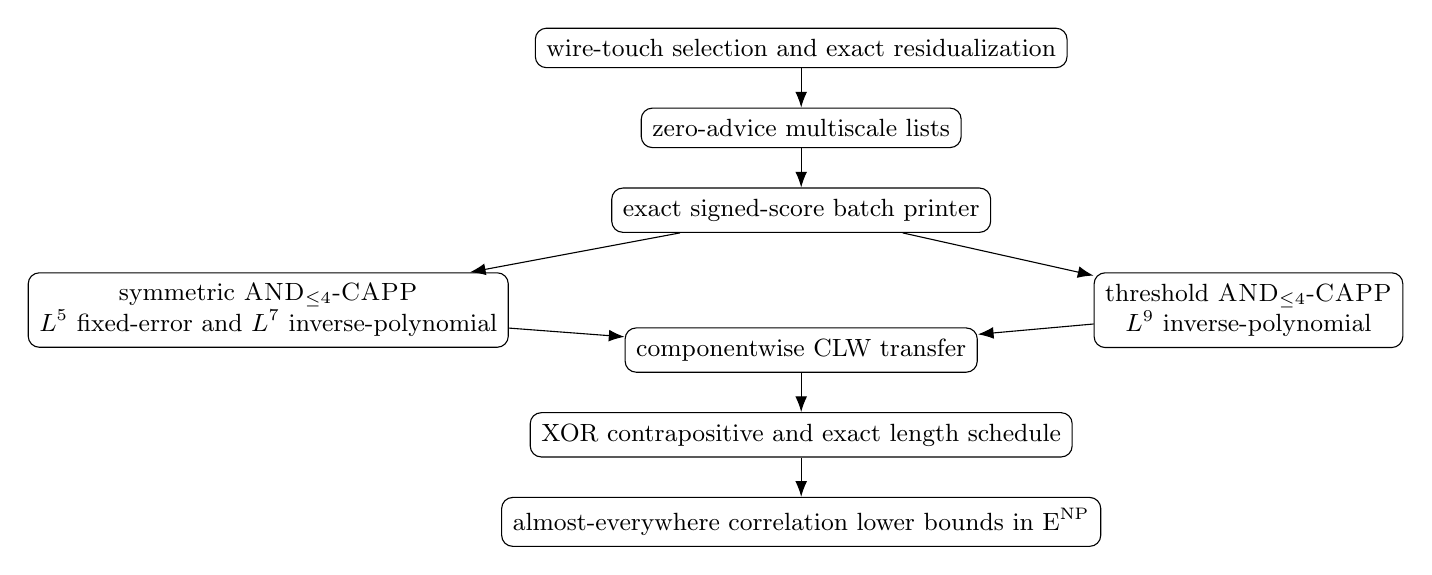
\begin{tikzpicture}[
  node distance=5mm and 13mm,
  every node/.style={draw,rounded corners,align=center,inner sep=4pt,
    font=\small},
  every path/.style={-{Latex[length=2mm]}}
]
\node (res) {wire-touch selection and exact residualization};
\node[below=of res] (lists) {zero-advice multiscale lists};
\node[below=of lists] (printer) {exact signed-score batch printer};
\node[below left=of printer] (sym) {symmetric \(\ANDfour\)-\CAPP\\
  \(L^5\) fixed-error and \(L^7\) inverse-polynomial};
\node[below right=of printer] (thr) {threshold \(\ANDfour\)-\CAPP\\
  \(L^9\) inverse-polynomial};
\node[below=12mm of printer] (transfer) {componentwise CLW transfer};
\node[below=of transfer] (xor) {XOR contrapositive and exact length schedule};
\node[below=of xor] (result) {almost-everywhere correlation lower bounds in \(\Eclass\)};
\draw (res) -- (lists);
\draw (lists) -- (printer);
\draw (printer) -- (sym);
\draw (printer) -- (thr);
\draw (sym) -- (transfer);
\draw (thr) -- (transfer);
\draw (transfer) -- (xor);
\draw (xor) -- (result);
\end{tikzpicture}
}
\caption{Dependency structure of the proof.}
\label{fig:proof-graph}
\end{figure}

The manuscript distinguishes imported facts from local work at every
seam. Finite threshold normalization, the qualitative provenance of the
disjoint exact-threshold conversion, exact Boolean rectangular
multiplication, the Gabber--Galil spectral estimate \cite{GG81} in the
normalization of \cite[Theorem 8.2]{HLW06}, the Rosser--Schoenfeld prime
estimate \cite[Theorem 4, eq. (3.14)]{RS62}, and the CLW/CW
verifier--refuter interfaces are
imported. The local crossing construction and all of its
quantitative bounds are replayed locally. Residualization, touching
selection, the zero-advice recurrence, walk amplification, exact row
construction, signed reduction, all resource ledgers, the componentwise
adapters, and the final scheduling are proved here.

\subsection{Proof overview}\label{sec:proof-overview}

Fix the supplier arity \(q\), let \(L_q=\lceil\log_2(q+2)\rceil\), and,
for a fixed positive integer \(\kappa\), keep \(K=\kappa L_q\) variables
live. For a bottom halfspace
\(X_i(y,z)\), define \(C_i(z)\) to be the indicator that
\(X_i(\cdot,z)\) is identically one and put

\[
Z_i=X_i\oplus C_i=X_i-C_i.
\]

Both constant-zero and constant-one restrictions now give \(Z_i=0\); the
removed contribution survives only in a scalar top offset. Choosing the
live set by conditional expectation over support incidences gives, on
every column,

\[
R=O(KW/q)
\]

touched carriers across all four input circuits. Complements and
fixed-radix clones reuse those supports. A pairwise nested hash then
gives a complete one-hot list of degree

\[
D_0=O(\sqrt R+L_q)
\]

with constant pointwise error and no advice. When inverse-polynomial
error is needed, componentwise majority along one explicit expander walk
multiplies degree by \(t=\Theta(L_q)\). A threshold top first becomes a
disjoint family of exact equations; a small-prime surrogate and
\(\tau=\Theta(L_q)\) radix digits use the same walk and the same
touched-carrier pool.

All list syntax is compiled into total Boolean rows before any column is
read. An occurrence-indexed truncated-binomial identity turns the parity
of the raw monomial count into one signed family of exact equations. The
exact signed-score printer evaluates all columns simultaneously. Its
only algebraic import is exact Boolean rectangular multiplication;
signed weights, ties, odd arity, and weighted dominance are derived
locally. The three resulting load inequalities and wire caps are collected
once, in \cref{tab:supplier-ledger}.

The algorithm may print \(q^{h_D}\) external rows. Choosing
\(\kappa>h_D+\sigma+10\) makes their column scans cost at most
\(2^q/q^\sigma\). Radix tuples, trace tuples, and exact-child choices are
internal syntax whose canonical expansion is paid once per row in

\[
T_{\mathrm{prep}}
\le
2^{O_D(dL_q+L_q^2+t)}
{}={}
2^{o(q)}.
\]

The truncated-binomial (BinLift) subsets are accounted for separately: they
form the signed exact-threshold occurrence family \(s_{\mathrm{gen}}\) in
\cref{thm:batch}, whose size is absorbed by the
\(2^{q-K}\poly(q)\) signed-score printing term. They are not included in
\(T_{\mathrm{prep}}\). The preprocessing term is added to the column time.
Every possible scalar
residue row is printed first; a column then selects one already printed
cell. These two orderings are what rule out an uncharged row family and
an adaptive choice of advice.

The lower-bound transfer works componentwise. A guessed real proof
coordinate has the form \(T=\sum_a\alpha_aC_a\), where each atom \(C_a\)
obeys the wire cap separately. Expanding the CLW Booleanity,
systematic-consistency, second-moment, and clause polynomials produces
conjunctions of at most four atoms. Term count controls the number of
calls, coefficient mass controls the required accuracy, and neither is
added to atom wires. Explicit parity coordinates cost only \(O(q)\)
wires for a symmetric top and \(O(q^2)\) for a threshold top.

One fixed weak machine freezes its data in the following order before it sees
a source length: the source transformations and two class presentations;
exact width padding and finite syntax envelopes; the target advantage and
target-class simulation exponent; the general-oracle exponent and Case-1
amplifier constants; the XOR power, componentwise envelopes, and validity
tolerance; and finally the supplier accuracy, saving, cap coefficients,
programs, and onsets. Only then is the finite union of the two class modes
fixed.

Outer-verifier duplicates are deleted before the PCPP because they form
a Boolean conjunction; indexed PCPP duplicates are retained because they
carry probability mass. Pointwise PCPP soundness is applied before
averaging, so every branch rejects a hierarchy no-instance. The CLW
refuter therefore produces, at every sufficiently large source length, a
yes-instance on which both modes reject. The deterministic honest PCPP
assignment defines one canonical Boolean proof-table function common to
the two modes. A nearby componentwise sum would create an accepting
branch, a contradiction.

Finally, the literal CLW XOR contrapositive turns this sum-hard function
into correlation hardness. For advantage \(n^{-c}\), take
\(k=\Theta_c(\log q)\) and retain the stronger reserve \(m^{-(c+1)}\) at
core arity \(m=k(q+O(\log q))\). A correlator becomes only a polynomial
family of literal restrictions of itself, so every atom keeps the same
absolute wire charge. The cubic arity dilation costs exactly three
logarithmic powers, taking the high-accuracy \(L^7/L^9\) supplier
denominators to the final \(L^{10}/L^{12}\) denominators. At fixed
advantage \(k=O(1)\), so the fixed-accuracy symmetric \(L^5\) and
threshold \(L^9\) rows pass through unchanged. A bounded-jump exact
schedule gives \(n/3\le m\le n/2\) at every sufficiently large target
length; hence \(m^{-(c+1)}<n^{-c}\) and a fixed coefficient absorbs the
target-to-core wire ratio. Canonical SAT recovery places the resulting
total language in \(E^{NP}\).

The delicate claims and their proof locations are therefore visible
before the technical proof begins:

\begin{center}
\small
\begin{tabularx}{\textwidth}{@{}p{0.31\textwidth}X@{}}
\multicolumn{2}{c}{\textbf{Audit map for the main proof seams.}}\\[0.4em]
\toprule
\textbf{Potential failure} & \textbf{Disposition} \\
\midrule
thin-gate explosion & charged by support incidences, not gate count \\
constant-one drift & exact residual \(Z_i=X_i-C_i\) and one scalar
offset \\
extra radix or child row & internal syntax versus external-row ledger \\
column-dependent advice & print every residue row before selecting a
cell \\
pointwise/average mismatch & pointwise list/prime bounds, then Fubini \\
hidden source-size factor & projection recovery and duplicate
outer-clause compaction \\
illegal aggregate circuit & componentwise caps; sums are never composed
for CAPP \\
length-dependent weak machine & explicit freeze order and fixed program
codes \\
wrong post-padding advantage & \(m^{-(c+1)}<n^{-c}\) reserve on
\(m\ge n/3\) \\
\bottomrule
\end{tabularx}
\end{center}

\section{Results and model}\label{sec:results-model}

All logarithms are base two, and

\[
L=L(n)=\lceil\log_2(n+2)\rceil.
\]

Physical wires count input-to-bottom incidences and top incidences in a
strictly layered simple-edge presentation. Parallel uses are explicit
occurrences, zero-weight inputs and zero top coefficients are deleted,
and constants are propagated before the resource is measured.

Some depth-two conventions also permit original input variables to feed
the top gate directly. Replace each such input-to-top incidence by a
fresh identity bottom threshold \(I_j(x)=\mathbf1[x_j\ge1]\) and one
incidence from \(I_j\) to the top, retaining the original top weight in
the threshold-top case. The symmetric-top case is the same unweighted
replacement. Each direct wire becomes exactly two strictly layered
wires, all other wires are unchanged, and the computed function is
identical. Consequently every theorem below also holds for this
skip-layer convention after shrinking its displayed positive wire
coefficient by a factor of two.

A threshold gate is \(\mathbf1[\sum_iw_ix_i\ge\theta]\), and a symmetric
gate is an arbitrary Boolean function of the unweighted number of its
accepting inputs. Both circuit classes have bottom threshold gates and
one top gate of the displayed type. If bottom occurrence \(G_i\) has
support \(\operatorname{supp}(G_i)\) and a nonzero top incidence, then

\[
W(C)
{}={}
\sum_i
\bigl(
|\operatorname{supp}(G_i)|+1
\bigr).
\]

Agreement means

\[
\operatorname{agr}(C,f)
{}={}
\Pr_{x\in\{0,1\}^n}[C(x)=f(x)].
\]

We use \(E^{NP}=\operatorname{DTIME}(2^{O(n)})^{NP}\).

Threshold gates may have arbitrary real weights semantically. For one
gate, first delete every zero-weight input and regard the remaining
variables as its support. On that finite Boolean cube, standard Muroga
normalization, equivalently \cite[Lemma 3.2]{CTW26}, supplies an
equivalent integer threshold description with every parameter in
\([-s^s,s^s]\), where \(s\) is that gate's retained
fan-in. Extend this description by zero on omitted variables. It need
not preserve the numerical weights; the point needed here is that it
introduces neither a new variable incidence nor another gate occurrence.

Throughout the algorithmic statements, \textbf{normalized} means this
support-first bounded integer representation, with a fixed canonical
binary syntax; a threshold top is normalized after zero top coefficients
are deleted, while a symmetric top is stored as its \((M+1)\)-bit count
lookup. At the displayed wire caps, the total normalized description
length is bounded by one fixed polynomial in the arity. Thus the
deterministic algorithms receive only a finite description with a
uniform polynomial-bit envelope. An alleged arbitrary-real circuit is
replaced existentially, gate by gate, before the transfer guesses it,
and literal restrictions, normalization, coefficient collection, and
constant propagation never increase physical wires. Fixing inputs
preserves both classes and cannot add wires. Output negation changes
only the symmetric lookup, or replaces a top inequality \(L\ge\theta\)
by \(-L\ge-\theta+1\), so it also preserves the class and wire count.

Both target classes contain parity below the displayed caps. For a
symmetric top, use identity bottoms and the parity lookup. For a
threshold top, use the staircase gates
\(T_j(x)=\mathbf1[\sum_ix_i\ge j]\) and the top gate

\[
\mathbf1\left[
\sum_{j=1}^n(-1)^{j+1}T_j(x)
\ge\frac12
\right].
\]

This uses \(O(n^2)\) physical wires, which is \(o(n^3/L^p)\) for every
displayed \(p\).

\subsection{Notation and terminology}\label{sec:notation}

For a Boolean circuit \(C\) on \(q\) inputs, \CAPP{} asks for an additive
estimate of \(\Pr[C(x)=1]\) under the uniform distribution. An
\(\ANDfour\)-\CAPP{} instance is the conjunction of at most four separately
represented circuits. We use \emph{supplier} for the deterministic
\(\ANDfour\)-\CAPP{} algorithm furnished to the lower-bound transfer, and
\emph{printer} for the batch subroutine that outputs an exact table of signed
scores. These terms name algorithms, not additional circuit classes.

\begin{center}
\small
\begin{tabularx}{\textwidth}{@{}p{0.23\textwidth}X@{}}
\multicolumn{2}{c}{\textbf{Local terminology and its standard algorithmic
meaning.}}\\[0.4em]
\toprule
Term & Meaning \\
\midrule
supplier & deterministic \(\ANDfour\)-\CAPP{} algorithm used by the
analysis-to-lower-bound transfer \\
printer & batched exact score evaluation by rectangular matrix
multiplication \\
carrier & a residual bottom-gate coordinate that can still vary on the live
variables \\
touching & incidence of a retained live variable in a bottom-gate support \\
residualization & subtracting the column-dependent constant-one indicator so
that every constant restricted gate has residual value zero \\
zero-advice list & an explicit multiscale counting-polynomial list whose
correct entry is selected from the input column, without guessed advice \\
\bottomrule
\end{tabularx}
\end{center}

The ``zero-advice'' qualifier distinguishes the local deterministic list from
the sampled probabilistic-polynomial construction of \cite{AW15}: every seed
is enumerated explicitly, and the correct row is selected only from the input
column.

\begin{center}
\small
\begin{tabularx}{\textwidth}{@{}lX@{}}
\multicolumn{2}{c}{\textbf{Principal parameters.}}\\
\multicolumn{2}{c}{\footnotesize Symbols reused as local functions or linear
forms are qualified in the corresponding section.}\\[0.4em]
\toprule
Symbol & Meaning \\
\midrule
\(n\) & final input length in the lower-bound theorems \\
\(q\) & native arity of a supplier call or padded verifier \\
\(L(r)\) & \(\lceil\log_2(r+2)\rceil\); we write \(L_q=L(q)\) \\
\(W(C)\) & physical-wire count of a normalized depth-two circuit \\
\(K=\kappa L_q\) & number of variables retained by the restriction;
\(\kappa\in\mathbb N\) is fixed \\
\(R\) & number of carrier coordinates touched by the live variables \\
\(D_0\) & degree of the unamplified multiscale list \\
\(D\) & requested accuracy exponent \\
\(d_{\rm row}\) & Boolean degree of a final printer row \\
\(\sigma\) & requested polynomial saving exponent \\
\(t,\tau\) & expander-walk length and number of radix digits \\
\(Q\) & modulus exponent in the truncated-binomial lift \\
\(h_D\) & exponent bounding the number of external rows \\
\(\rho_{\rm coef}\) & exponent bounding coefficient mass in the transfer \\
\(C_{\rm batch}\) & absolute constant in the exact batch theorem \\
\(C_{\rm clk}\) & polynomial-clock exponent in the CLW transfer \\
\bottomrule
\end{tabularx}
\end{center}

The circuit-analysis result is a standalone algorithmic contribution. A
\emph{normalized} threshold gate is reduced to its nonzero support of size
\(s\) and represented by integer parameters in \([-s^s,s^s]\), as supplied
by \cite{MTT61}; see also \cite[Lemma 3.2]{CTW26}. We fix one canonical
binary syntax. A threshold top is normalized on its retained bottom
occurrences, while a symmetric top is represented by its count lookup.

\begin{theorem}[Inverse-polynomial fourfold supplier]
\label{thm:supplier-inverse}
For every fixed accuracy exponent \(D>0\) and requested polynomial saving
exponent \(\sigma>0\), there are constants
\(a_{\mathrm S},a_{\mathrm T}>0\) and deterministic algorithms with the
following behavior. Given at most four normalized \(q\)-input circuits from
one of the two named classes, the algorithm estimates their conjunction
probability to error at most \(q^{-D}\) in total time
\[
\frac{2^q}{q^\sigma},
\]
including input processing, whenever every input has, respectively,
\[
W(C_i)\le a_{\mathrm S}\frac{q^3}{L_q^7}
\qquad\text{or}\qquad
W(C_i)\le a_{\mathrm T}\frac{q^3}{L_q^9}.
\]
The constants may depend on \(D\) and \(\sigma\).
\end{theorem}

\begin{theorem}[Fixed-accuracy symmetric supplier]
\label{thm:supplier-fixed}
For every fixed \(0<\epsilon<1/2\) and \(\sigma>0\), there are a constant
\(a_{\mathrm S}^{\mathrm{fix}}>0\) and a deterministic algorithm that
estimates the conjunction probability of at most four normalized
\(q\)-input \(\SYMTHR\) circuits to additive error at most \(\epsilon\) in
total time \(2^q/q^\sigma\), including input processing, whenever every
input satisfies
\[
W(C_i)\le a_{\mathrm S}^{\mathrm{fix}}\frac{q^3}{L_q^5}.
\]
The constant may depend on \(\epsilon\) and \(\sigma\).
\end{theorem}

The proofs of \cref{thm:supplier-inverse} and \cref{thm:supplier-fixed} occupy
Appendices~\ref{appendix-a-the-residualized-and-four-suppliers} and
\ref{appendix-b-exact-signed-score-printing}. The lower-bound transfer begins
in \cref{sec:transfer}.

\begin{theorem}[Inverse-polynomial correlation hardness]
\label{thm:main-inverse}
For every fixed \(c>0\), there exist a language \[
F_c\in E^{NP}
\] and constants \(b_{\mathrm S,c},b_{\mathrm T,c}>0\) such that the
following holds at every sufficiently large input length \(n\).

If \(C\in\mathrm{SYM}\circ\mathrm{THR}\) and \[
W(C)\le b_{\mathrm S,c}\frac{n^3}{L^{10}},
\] then \[
\operatorname{agr}(C,(F_c)_n)<\frac12+n^{-c}.
\]

If \(C\in\mathrm{THR}\circ\mathrm{THR}\) and \[
W(C)\le b_{\mathrm T,c}\frac{n^3}{L^{12}},
\] then the same correlation inequality holds.
\end{theorem}

The same language works for both classes. The language and the two
positive constants are joint existential witnesses; the construction
freezes both class caps before freezing the one finite-mode weak
machine.

\begin{corollary}[Every fixed multiplier]\label{cor:every-multiplier}
For the same \(F_c\),
both of the following hold for every fixed \(A>0\) and every
sufficiently large \(n\): \[
W(C)\le A\frac{n^3}{L^{11}}
\quad\Longrightarrow\quad
\operatorname{agr}(C,(F_c)_n)<\frac12+n^{-c}
\] for \(\mathrm{SYM}\circ\mathrm{THR}\), and \[
W(C)\le A\frac{n^3}{L^{13}}
\quad\Longrightarrow\quad
\operatorname{agr}(C,(F_c)_n)<\frac12+n^{-c}
\] for \(\mathrm{THR}\circ\mathrm{THR}\).
\end{corollary}

Indeed \(A/L\) is eventually smaller than the corresponding fixed
positive constant. The same observation proves a more precise
consequence: for every function \(u(n)\to\infty\), with no
constructibility assumption,

\[
A\frac{n^3}{L^{10}u(n)}
\]

and

\[
A\frac{n^3}{L^{12}u(n)}
\]

are defeated by this same language after a \(u\)-dependent onset.

\begin{theorem}[Fixed advantage]\label{thm:main-fixed}
For every fixed
\(0<\gamma<1/2\), there exist a common language \(F_\gamma\in E^{NP}\)
and positive constants \(b_{\mathrm S,\gamma},b_{\mathrm T,\gamma}\)
such that, for every sufficiently large \(n\), agreement at least
\(1/2+\gamma\) with \((F_\gamma)_n\) implies
\[
W(C)>b_{\mathrm S,\gamma}\frac{n^3}{L^5}
\]
for \(C\in\SYMTHR\), and
\[
W(C)>b_{\mathrm T,\gamma}\frac{n^3}{L^9}
\]
for \(C\in\THRTHR\).
\end{theorem}

Thus the same fixed-advantage language defeats every fixed multiplier at
denominators \(L^6\) and \(L^{10}\). The unequal exponents reflect two
real compiler costs: inverse-polynomial amplification costs two
logarithmic powers after printer squaring, while exact radix lookup for
an arbitrary threshold top costs two more.

\section{Why this is not a moving-delta
corollary}\label{3-why-this-is-not-a-moving-delta-corollary}

The fixed-\(\delta\) theorem says, separately for every fixed
\(\delta>0\), that a language is hard at wire scale \(n^{3-\delta}\). It
gives no uniform relation among the language, algorithm, constants, and
onset as \(\delta\downarrow0\). This logical gap is large enough to
contain every polylogarithmic endpoint.

For example,

\[
h(n)=\frac{n^3}{\exp(\sqrt{\log n})}
\]

eventually dominates \(n^{3-\delta}\) for each fixed \(\delta>0\), but
satisfies

\[
h(n)=o\left(\frac{n^3}{(\log n)^K}\right)
\]

for every fixed \(K\). Hence all fixed-power statements are compatible
with the complete failure of every explicit logarithmic statement.

Nor can one safely schedule row \(j\) at length \(n\) without
quantitative onset control. The theorem permits the onset of row \(j\)
to occur after the finite interval in which its bound exceeds the
desired \(n^3/L^K\) scale. For correlation, selector packaging is
additionally invalid because all of a correlator's
signed bias may concentrate on the ineligible rows. The explicit-log
theorem below instead fixes one uniform supplier and one refuter
construction.

\section{The residualized wire-sensitive
supplier}\label{4-the-residualized-wire-sensitive-supplier}

Fix a live coordinate set \(I\). Write a normalized bottom halfspace as

\[
X_i(y,z)
{}={}
\mathbf1\left[
\sum_{j\in I}w_{ij}y_j+
\sum_{j\notin I}w_{ij}z_j
\ge\theta_i
\right].
\]

Let

\[
m_i^-=\sum_{j\in I:w_{ij}<0}w_{ij}
\]

and define

\[
C_i(z)
{}={}
\mathbf1\left[
\sum_{j\notin I}w_{ij}z_j
\ge\theta_i-m_i^-
\right].
\]

Then \(C_i(z)=1\) exactly when \(X_i(\cdot,z)\) is identically one. In
particular \(C_i\le X_i\), and

\[
Z_i=X_i\oplus C_i=X_i-C_i
\]

is Boolean, vanishes whenever the restricted gate is constant, and
equals \(X_i\) whenever it is nonconstant. Over \(\mathbb F_2\) this is
a degree-one substitution. The carrier pool grows by only a constant
factor and no residual coordinate has fixed-one drift.

For a symmetric top, the omitted contribution is the scalar

\[
F(z)=\sum_iC_i(z).
\]

For up to four threshold-top outputs, \cref{prop:child-tuples} converts each
top gate to a disjoint OR of polynomially many exact equations.
Expanding the desired conjunction chooses at most one child per input
circuit; a domination-base stack turns each child tuple into one exact
equation. Averaging its reductions modulo all primes below an explicit
polynomial cutoff gives a pointwise inverse-polynomial surrogate in
which every modular predicate is one polynomial-range nonnegative score.
Residualization moves the constant-one contribution into one scalar
residue \(f_{g,p}(z)\) for that equation and prime. The algorithm prints
every possible residue row before the column scan and then selects the
correct row; it never enumerates an independent drift value for every
level or digit.

Let \(q\) now denote supplier arity and put \(L_q=L(q)\). Fix a positive
integer \(\kappa\). TouchingSelect, the conditional-expectation selection
procedure of
\cref{a4-touching-and-multiscale-list}, finds one live set of size

\[
K=\kappa L_q
\]

for which every restriction column has at most

\[
R=O\left(\frac{KW}{q}\right)
\]

nonconstant carriers across the union of the at most four input
circuits. Indeed, a support of size \(f\) is touched by a random
\(K\)-set with probability at most \(Kf/q\), and conditional expectation
derandomizes the summed support bound. Every gate nonconstant on any
column must be touched.

Take \(J=\lceil2L_q\rceil\). \Cref{lem:window-indicators} and
\cref{lem:zero-advice-list} print the
consecutive-window indicators and the exact downward recurrence for a
pairwise multiscale list of degree

\[
D_0=O(\sqrt R+L_q)
\]

and seed entropy \(O(L_q)\). Moreover \(R2^{-J}=O(L_q^{1-p})=o(1)\) at
every displayed supplier denominator \(p\ge5\), so the lemma's finite
terminal premise holds from a sufficiently large arity onward. There is
no bad-column term and no drift-advice entropy.

\subsection{Direct symmetric top}\label{41-direct-symmetric-top}

For constant final error, multiply at most four scalar list outputs. The
exact batch theorem in \cref{a12-exact-score-batch-theorem-and-additive-preprocessing} first converts bottom thresholds
disjointly to exact equations, canonically reduces the squarefree
polynomial, and applies the occurrence-indexed truncated-binomial lift.
\cref{thm:signed-printer} derives the required signed table from
Williams's stated exact Boolean rectangular product by
local binary slicing and weighted dominance. Its leading closure term is

\[
K D_0 L_q\lesssim q.
\]

After squaring the \(\sqrt R\) term, the normalized master parameter is

\[
\Xi_{\mathrm S,\mathrm{const}}
{}={}
\Theta\left(
\frac{W K^3L_q^2}{q^3}
\right).
\]

At \(K=\kappa L_q\), a sufficiently small positive coefficient times
\(q^3/L_q^5\) makes this parameter smaller than the printer constant.

For error \(q^{-D}\), take the odd walk length

\[
t=2\left\lceil\frac{C_D L_q}{2}\right\rceil+1
\]

walk on a fixed power of the Margulis expander over the exact pairwise
hash-seed space. Componentwise majority reduces error to
\(2^{-\Omega(t)}\) while multiplying degree by \(t\) and adding only
\(O_D(L_q)\) seed bits. The inverse-polynomial direct master is

\[
\Xi_{\mathrm S,\mathrm{inv}}
{}={}
\Theta_D\left(
\frac{W K^3t^2L_q^2}{q^3}
\right).
\]

It closes at a sufficiently small positive multiple of

\[
\frac{q^3}{L_q^7}.
\]

\subsection{Threshold top}\label{42-threshold-top}

Binary or fixed-radix reconstruction uses

\[
\tau=\Theta_D(L_q)
\]

digit lists over the same distinct-carrier pool. Touching is charged
once, not once per digit. Walk majority is applied before the exact
modular-radix lookup. The conjunction of up to four outputs was already
converted to a polynomial family of stacked top equations, and each
equation-prime row has exactly one pre-radix score.

Writing \(d_{\rm row}\) for the final Boolean row degree (and retaining
\(D\) only for the requested accuracy exponent), the composed degree is

\[
d_{\rm row}=O_D(t\tau D_0),
\]

and the master parameter is

\[
\Xi_{\mathrm T}
{}={}
\Theta_D\left(
\frac{W K^3t^2\tau^2L_q^2}{q^3}
\right).
\]

In all three masters, only the \(\sqrt R\) part of \(D_0\) depends on
the wire cap. The additive \(L_q\) part and the batch
theorem's additive \(K+\log(Q+1)+L_q\) terms contribute
only fixed powers of \(L_q=o(q)\) after \(Q=K+1\); they impose no
additional denominator.

Thus a sufficiently small positive multiple of

\[
\frac{q^3}{L_q^9}
\]

supports arbitrary fixed inverse-polynomial accuracy. Enlarging the
explicit prime cutoff makes each nonzero stacked equation pass on a
\(q^{-D-O(1)}\) fraction of primes, while increasing the walk constant
makes every modular row pointwise reliable to the same scale. The
polynomial child-tuple count is paid by these accuracy constants, not by
changing the logarithmic exponent.

\subsection{Selectable polynomial saving and additive
preprocessing}\label{43-selectable-polynomial-saving-and-additive-preprocessing}

The constants matter. Let \(D\) be the requested accuracy and let
\(\sigma>0\) be the requested saving exponent. Stacked-equation indices,
primes, scalar residues, expanded walk seeds, and constant input-side
labels form only \(q^{h_D}\) \textbf{external rows} for one fixed
\(h_D\). Choose

\[
\kappa>h_D+\sigma+10.
\]

Then the combined external column phases have time at most

\[
\frac{2^q}{q^\sigma}
\]

after every polynomial overhead.

The exact radix lookup inside one threshold row has up to

\[
(b_0M+1)^{\tau}
{}={}
2^{O_D(L_q^2)}
\]

internal tuple monomials. These are not external calls. For each fixed
external row, the exact batch theorem charges their canonical expansion
in

\[
T_{\mathrm{prep}}
\le
2^{O_D(dL_q+L_q^2+t)},
\]

where \(d\) is the final Boolean row degree. The truncated-binomial
counter is used with the minimal modulus exponent \(Q=K+1\): this
uniquely recovers a count in \([0,2^K]\) and makes the leading printer
constraint \(K d L_q=O(q)\). Since the strict printer inequality gives
\(dL_q=O(q/K)=O(q/L_q)\),

\[
\log_2T_{\mathrm{prep}}
{}={}
O_D(q/L_q+L_q^2)
=o(q).
\]

There are \(q^{h_D}\) external rows, so the complete preprocessing
charge is

\[
q^{h_D}T_{\mathrm{prep}}
{}={}
2^{o(q)}.
\]

It is therefore eventually below \(2^q/q^\sigma\). This charge is added
to, and never multiplied by, the \(2^{q-K}\) enumeration of columns. The
printer loads grow like a fixed multiple of

\[
\sqrt a\,\kappa^{3/2}
\]

when \(W=a q^3/L_q^p\). Choosing

\[
0<a\le a_0(D)\kappa^{-3}
\]

therefore restores the printer inequality and proves the
inverse-polynomial guarantees in \cref{thm:supplier-inverse}.

In addition, for every fixed \(0<\epsilon<1/2\) and \(\sigma>0\),
\cref{thm:supplier-fixed} gives a positive constant \(a_{\mathrm S}^{\mathrm{fix}}\)
and a deterministic additive-\(\epsilon\) estimator for symmetric-top
AND-four at total time \(2^q/q^\sigma\) on

\[
W\le a_{\mathrm S}^{\mathrm{fix}}\frac{q^3}{L_q^5}.
\]

This is the formal supplier used by the symmetric half of \cref{thm:main-fixed}.
The threshold half continues to use the \(L_q^9\) inverse-polynomial
supplier because its polynomial child-tuple sum requires
inverse-polynomial primitive accuracy.

\subsection{The deterministic
estimators}\label{44-the-deterministic-estimators}

The full estimators are defined once in
\cref{a13-native-threshold-and-four-compiler-and-explicit-estimators}. The
important ordering is that every seed-and-offset row is printed before a
column computes its residual offset and selects an existing cell. For every
fixed input and seed, both the selected row and its target are bits, including
on malformed one-hot lists. Fubini therefore bounds the symmetric estimator's
error by the joint input-seed list-failure probability; no seed must work on
every input. For a threshold top, the disjoint-child identity is pointwise
zero or one, and the prime and list errors are chosen below the inverse of the
polynomial child-tuple count. Fubini and the triangle inequality then give
the claimed \(q^{-D}\) error without discarding columns or performing a
signed affine recombination.

\subsection{Integrated supplier conservation
certificate}\label{45-integrated-supplier-conservation-certificate}

The supplier is one composition theorem, not a list of independently
invoked subroutines. The following table records the complete leading
ledger after \(K=\kappa L_q\), \(R=O(KW/q)\), and
\(D_0=O(\sqrt R+L_q)\). Here \(t=\Theta_D(L_q)\) is the walk length and
\(\tau=\Theta_D(L_q)\) is the number of radix digits.

\begin{table}[t]
\centering
\caption{Complete leading supplier ledger.}
\label{tab:supplier-ledger}
\small
\begin{tabular}{@{}llll@{}}
\toprule
\textbf{Mode} & \textbf{Extra} & \textbf{Load} & \textbf{Cap} \\
\midrule
SYM, fixed & none & \(WK^3L_q^2/q^3\) & \(a q^3/L_q^5\) \\
SYM, \(q^{-D}\) & \(t\) & \(WK^3t^2L_q^2/q^3\) & \(a q^3/L_q^7\) \\
THR, \(q^{-D}\) & \(t\tau\) & \(WK^3t^2\tau^2L_q^2/q^3\) &
\(a q^3/L_q^9\) \\
\bottomrule
\end{tabular}
\end{table}

At each displayed cap the leading load is \(\Theta_D(a\kappa^3)\). The
parameters are chosen in this order: first \(D\) and \(\sigma\); then the
conversion, prime, radix, and walk constants; then the external-row exponent
\(h_D\); next \(\kappa>h_D+\sigma+10\); and finally a positive cap
coefficient \(a\le a_0(D)\kappa^{-3}\) and one finite onset.

The distinction between one row and all rows is equally important.

\begin{itemize}
\item
  \textbf{One external row.} It fixes one child tuple \(g\), prime
  \(p\), walk seed \(e\), and scalar residue \(f\), and is charged one
  complete \(2^{q-K}\)-column score table.
\item
  \textbf{Internal row syntax.} Radix tuples, trace tuples, exact-child
  choices, and their canonical polynomial expansion are charged in
  \(T_{\mathrm{prep}}=2^{O_D(dL_q+L_q^2+t)}\) before that
  row's column scan. Live assignments and BinLift subsets generate the
  signed occurrence family \(s_{\mathrm{gen}}\), which is bounded by
  \(2^{(q-K)/100}\) and paid inside the signed-score printing term of
  \cref{thm:batch}.
\item
  \textbf{All external rows.} There are at most \(q^{h_D}\) choices, so
  both one-row charges are multiplied by \(q^{h_D}\) exactly once.
\item
  \textbf{Column-dependent data.} The actual residual offset
  \(f_{g,p}(z)\) selects one cell only after every possible residue row
  has been printed.
\end{itemize}

The strict printer inequality gives \(dL_q=O(q/L_q)\), so

\[
q^{h_D}T_{\mathrm{prep}}
{}={}
2^{o(q)}.
\]

The column tables cost at most

\[
q^{h_D}2^{q-K}\operatorname{poly}(q)
\le
\frac{2^q}{q^\sigma}
\]

by the choice of \(\kappa\). The preprocessing term is \textbf{added} to
this quantity and satisfies the same final bound after the finite onset.
No radix tuple or exact-child tuple is also counted as an external row,
and no scalar offset is chosen before its complete table exists. This
simultaneously closes the row-multiplicity, hidden-logarithm, and
adaptive-row seams in the three-mode supplier composition.

\section{Componentwise CLW transfer with polynomial
saving}\label{sec:transfer}

The transfer uses the following source/local boundary.

\begin{itemize}
\item
  \textbf{CLW outer verifier.} The published contract gives one native
  random/address width, projection queries, a 3CNF predicate, perfect
  completeness, and \(N^{-10}\) no-instance acceptance. Locally we prove
  exact width padding, projection-table recovery, duplicate outer-clause
  deletion, and compact substitution.
\item
  \textbf{CLW/CW pointwise PCPP.} The published contract gives a
  deterministic honest assignment on a true input, soundness against
  every auxiliary assignment on a false input, and systematic parity
  coordinates. Locally we prove the componentwise validity polynomials,
  native parity atoms, occurrence aliases, and the acceptance midpoint.
\item
  \textbf{CLW fixed-machine refuter.} The published contract gives a
  disagreement at every sufficiently large source length against one
  fixed weak machine. Locally we construct one finite union of class
  modes and prove one-sidedness, common-function extraction, and
  canonical recovery.
\item
  \textbf{CLW XOR contrapositive.} The published contract gives the
  literal \(\varepsilon_k\)-dependent restriction-sum envelope. Locally
  we prove supported-versus-carried cap retyping, the three-log arity
  dilation, and the padding-safe advantage reserve.
\item
  \textbf{CLW/STV worst-case amplification.} The published contract
  turns size-\(S(q)\) worst-case hardness into an \(O(q)\)-variate
  output hard at size \(S(q)^{1/c_{\mathrm{STV}}}\) and advantage
  \(S(q)^{-1/c_{\mathrm{STV}}}\). Locally we prove one
  branch-independent arity envelope, choose \(G\) before \(k\) without
  circularity, and give the exact target schedule.
\end{itemize}

Nothing in the local column silently strengthens a published theorem. In
particular, outer duplicate clauses may be deleted because they form an
ordinary conjunction, whereas PCPP indexed-clause multiplicities are
retained because they define an acceptance distribution.

The objects passed across the splice have the following literal types.

\begin{itemize}
\item
  \textbf{Padded outer verifier.} Its varying input is
  \(u\in\{0,1\}^q\), where \(q=C_{\mathrm{clk}}\log N+O(\log\log N)\), and it has
  polynomially many projection queries. It defines the ordinary
  substituted circuit.
\item
  \textbf{Guessed general oracle.} It is a \(q\)-input fan-in-two
  circuit of size at most \(q^G\). It is substituted before the PCPP and
  is never sent to CAPP.
\item
  \textbf{PCPP coordinate function \(T_X\).} On \(u\in\{0,1\}^q\) it is
  one rational componentwise sum with fixed term, mass, and
  coefficient-bit envelopes. Every occurrence of variable \(X\) aliases
  this same function.
\item
  \textbf{Carried atom.} Before address fixing it has
  \(q_0=q+O(\log q)\) inputs and satisfies
  \(W\le B_{\mathfrak C}(q_0)\). Literal address fixing returns it to
  native arity without increasing wires.
\item
  \textbf{Systematic coordinate.} It is a native \(q\)-input explicit
  parity with \(O(q)\) wires for a symmetric top or \(O(q^2)\) wires for
  a threshold top. It enters as a separate cheap atom.
\item
  \textbf{CAPP input.} It is a native \(q\)-input conjunction of at most
  four atoms, each separately below \(A_{\mathfrak C}(q)\). It estimates
  one monomial of a validity or clause polynomial.
\item
  \textbf{Case-2 hard table \(f\).} It is a total Boolean function on
  \(q_0\) bits, with malformed addresses set to zero, and is the common
  componentwise-sum target for both class modes.
\item
  \textbf{XOR core.} It has \(m=kq_0\) inputs, where
  \(k=\Theta_c(\log q)\) or \(O_\gamma(1)\), and converts sum-hardness
  into correlation hardness.
\end{itemize}

The resource distinction in the CAPP row is crucial: coefficient mass
and term count govern estimation accuracy and the number of calls, but
the wire cap is imposed \textbf{componentwise} on each atom. No linear
sum is composed into one larger circuit and no sum of atom wires is
charged to a supplier call.

The fixed-machine quantifier order is as follows. Fix the published source
transformations and class presentations, then the exact-width padding and
parsers, the target advantage and simulation exponent, the general-oracle
exponent and amplifier constants, the XOR power and componentwise envelopes,
the validity tolerance and supplier parameters, the supported and carried
coefficients, and the supplier programs. Fix the finite union-machine code
only after these choices. The source length, refuter word, branch guesses, and
canonical hard objects are chosen afterward.

In particular, no program, cap coefficient, onset, term envelope, or
parser inside the weak machine depends on the current source length or
on a guessed circuit.

For a base class \(\mathfrak C\), define

\[
\operatorname{Lin}_q(B,J,\Lambda)
\]

to contain rational sums

\[
P(x)=\sum_{a=1}^s\alpha_a C_a(x)
\]

with

\[
s\le J,
\qquad
\sum_a|\alpha_a|\le\Lambda,
\qquad
W(C_a)\le B
\]

for every individual atom; all rational coefficients have polynomial bit
length. When the transfer writes \(P\in[0,1]\operatorname{Lin}_q\), it
additionally imposes \(0\le P(x)\le1\) pointwise. This is a semantic
property of the approximator produced by the XOR contrapositive, not a
promise that the weak machine tries to decide: the machine permits every
syntactically bounded rational sum, and its one-sided soundness proof
handles arbitrary real values through the Booleanity and second-moment
tests. A degree-four expression in such sums and constants expands into
at most \((J+1)^4\) AND-four calls. Its propagated additive error is at
most

\[
\eta(1+\Lambda)^4,
\]

while \((J+1)^4\) affects only time. No sum of atom wires is ever
presented to CAPP.

\cref{sec:published-interfaces} restates the four published CLW/CW/STV semantic interfaces,
and \cref{c10-full-componentwise-weak-machine-replay} replays the weak machine. Before applying the
pointwise PCPP, the local compaction lemma recovers the promised
projection table and deletes repeated outer 3CNF clauses. Since the
outer predicate has only \(t_{\rm out}=\operatorname{poly}(q)\) answer
variables, at most
\(8\sum_{j\le3}\binom{t_{\rm out}}j=q^{O(1)}\) distinct clauses remain.
Thus the substituted circuit has size \(q^{O(1)}\); no source-level
\(\operatorname{poly}(N)\) representation factor enters the PCPP witness
or call count. PCPP clause multiplicities, by contrast, are retained
because that theorem measures the fraction of its indexed list.

For an auxiliary proof occurrence the machine tests

\[
T_{ij}^2(1-T_{ij})^2,
\]

for a systematic occurrence it tests

\[
(\operatorname{Enc}_s-T_{ij})^2,
\]

and in both cases it also bounds \(\mathbb E[T_{ij}^2]\). These are
degree-four expressions in the guessed sums. The PCPP clause pool,
guessed proof descriptions, term counts, witness length, coefficient
masses, and coefficient-bit bounds are a finite list of fixed polynomial
envelopes once the target advantage exponent is fixed. They are frozen
before the weak machine; no one machine is claimed to cover all
polynomial envelopes. Let \(q^{p_{\mathrm{call},c}}\) bound the number
of analysis calls and their remaining polynomial overhead, write
\(2^q\le T(N)q^{d_{\mathrm{pad}}}\), and let the coefficient mass be at
most \(q^{\rho_{\mathrm{coef}}}\). Request

\[
D>4\rho_{\mathrm{coef}}+10
\]

and

\[
\sigma>p_{\mathrm{call},c}+d_{\mathrm{pad}}+10
\]

from \cref{thm:supplier-inverse}. Then all ordinary validity calls together cost at most
\(T(N)/q^{10}\).

A systematic code coordinate is an explicit parity of at most \(q/2\)
variables. Compile it directly into the selected target class: identity
bottoms plus a symmetric lookup use \(O(q)\) wires, while cumulative
threshold bottoms plus alternating top weights use \(O(q^2)\) wires.
Thus the parity atom is eventually below every supported cap
\(a_{\mathfrak C}q^3/L(q)^p\). Expanding \((\operatorname{Enc}_s-T)^2\)
now uses only native-arity conjunctions of at most two carried/parity
atoms, and all systematic tests cost

\[
q^{p_{\mathrm{call},c}}\frac{2^q}{q^\sigma}
\le
T(N)q^{-10}.
\]

The absolute atom charge is unchanged. Distinguish the
supplier-supported cap

\[
A_{\mathfrak C}(q)=a_{\mathfrak C}\frac{q^3}{L(q)^p}
\]

from the carried cap
\(B_{\mathfrak C}(q_0)=b_{\mathfrak C}q_0^3/L(q_0)^p\) on the addressed
function, where \(q_0=q+O(\log q)\). Choosing
\(b_{\mathfrak C}\le a_{\mathfrak C}/64\) gives

\[
B_{\mathfrak C}(q_0)\le A_{\mathfrak C}(q)
\]

eventually; before the coefficient factor, this arity ratio is only
\(1+o(1)\). Thus address restriction is legal, while systematic parity
never changes the native arity. This is why the theorem obtains a
positive constant rather than every constant at the boundary.

The native verifier width is padded locally to the exact value

\[
q(N)
{}={}
\left\lceil\log_2T(N)\right\rceil
{}+{}
A_{\mathrm{pad}}
\left\lceil\log_2(\log_2T(N)+2)\right\rceil
{}+{}
A_{\mathrm{pad}}.
\]

The added random bits are ignored and native proof addresses receive a
zero suffix, so completeness, acceptance fractions, and projection
typing are unchanged; moreover \(2^q/T(N)=q^{O(1)}\). The complete
witness has \(q^{O_c(1)}=o(N)\) bits and is eventually below the
refuter's \(N/10\) bound. Let \(d_{\mathrm{ver}}\) bound
source construction, projection-table recovery, outer-clause compaction,
and substitution. Choose the polynomial clock exponent with
\(C_{\mathrm{clk}}>d_{\mathrm{ver}}+2\):

\[
T(N)=N^{C_{\mathrm{clk}}}
\]

The compacting work is \(N^{d_{\mathrm{ver}}}q^{O(1)}=o(T(N))\), while
choosing the requested CAPP saving beyond the fixed call and padding
exponents makes the complete analysis phase at most \(T(N)/q^{10}\).
Hence the machine is genuinely \(o(T(N))\). Freeze a rational validity
tolerance \(\zeta>0\), and require every propagated estimate to have
error below both \(\zeta\) and one twentieth of the PCPP
completeness--soundness gap. The first bound makes the Booleanity and
second-moment thresholds sound; the second protects the acceptance
midpoint. The machine estimates the arithmetized clause mean and accepts
only above that midpoint. On a hierarchy NO word, outer soundness,
pointwise PCPP soundness, and validity rounding keep every branch
strictly below it. The fixed-machine refuter consequently produces, at
every sufficiently large source length, a YES word on which every class
mode rejects.

At that conflict, either Case 1 supplies a general-circuit-hard oracle,
or Case 2 chooses the lexicographically first eligible succinct general
oracle before the class mode. In Case 2, the PCPP's
fixed deterministic honest-assignment algorithm defines one canonical
Boolean proof family and hence

\[
f(i,j,u)=\widehat T_{ij}(u),
\]

with malformed indices mapped to zero. If an eligible componentwise sum
approximated \(f\), occurrence averaging would construct a valid
accepting proof in that class mode without increasing any
atom's wires, contradicting rejection. Thus the same
Case-2 proof-table function is far from componentwise sums of both
circuit classes.

\section{XOR amplification and the three-log
dilation}\label{6-xor-amplification-and-the-three-log-dilation}

For target advantage \(n^{-c}\) after padding, let

\[
\varepsilon_k=(1-\zeta)^{k-1}(1/2-\zeta)
\]

be the source parameter in CLW's XOR contrapositive and
take

\[
k=A_{c+1}\lceil\log_2(q+2)\rceil,
\]

where the fixed \(A_{c+1}\) is large enough that
\(\varepsilon_k\le q^{-(c+2)}\). The final Case-2 function has arity

\[
m=k(q+O(\log q))=\Theta_c(q\log q).
\]

Because \(m=\Theta_c(q\log q)\), eventually

\[
\varepsilon_k
\le q^{-(c+2)}
\le m^{-(c+1)}.
\]

The term-count and coefficient-mass envelopes are evaluated at the
actual source value \(\varepsilon_k=q^{-O_c(1)}\); they remain fixed
polynomials in \(q\). This avoids silently substituting a different
advantage into CLW's quantitative bound. The one-power
\(m^{-(c+1)}\) reserve is what makes the later padding to target arity
\(n\) preserve the theorem's stricter threshold
\(n^{-c}\).

A correlator for the \(k\)-fold XOR yields polynomially many literal
restrictions of that correlator as the atoms of one approximate linear
sum. No XOR gate is composed on top of an atom.

Suppose first that a symmetric-top correlator has

\[
W(C)\le b_{\mathrm S,c}\frac{m^3}{L(m)^{10}}.
\]

Every restricted atom has the same absolute charge, and

\[
W(C_a)
\le
O_c(b_{\mathrm S,c})
\frac{q^3(\log q)^3}{(\log q)^{10}}
{}={}
O_c(b_{\mathrm S,c})
\frac{q^3}{(\log q)^7}.
\]

Choose \(b_{\mathrm S,c}\) below the fixed supplier coefficient after
all arity constants. The atom is legal. The threshold-top calculation is
identical:

\[
\frac{m^3}{L(m)^{12}}
{}={}
O_c\left(\frac{q^3}{L(q)^9}\right).
\]

Thus exactly three logarithmic powers pay the cubic arity dilation. No
fourth power is needed for the fixed-positive theorem. A fourth power
converts the fixed positive constant into every fixed multiplier,
proving \cref{cor:every-multiplier}.

For fixed advantage, \(k=O_\gamma(1)\) and \(m=\Theta_\gamma(q)\).
Choose this constant large enough not only to drive the XOR residual
advantage below \(\gamma\), but also to dominate the fixed output-arity
constant in the Case-1 amplifier of \cite[Lemma 3.9]{CLW20} and
\cite[Theorem 24]{STV01}. There is no logarithmic arity dilation, so the supplier exponents
themselves become the final exponents in \cref{thm:main-fixed}.

\section{\texorpdfstring{Case 1, every length, and
\(E^{NP}\)}{Case 1, every length, and E\^{}\{NP\}}}\label{7-case-1-every-length-and-enp}

If no small general oracle makes the outer verifier a tautology, apply
the exact Case-1 contract stated as \cref{fact:case-one-amplifier}. It gives a function on
at most \(c_{\mathrm{amp}}q\) variables that is hard at both circuit
size and advantage exponent \(G/c_{\mathrm{STV}}\), and its complete
truth table is computable from the hard outer-oracle table in
\(2^{O(q)}\) time. After finite normalization, bottom and top threshold
gates have polynomial-bit descriptions, while a symmetric top has an
\(M+1\)-entry lookup. Binary addition and comparison therefore simulate
a displayed-cap circuit by a fan-in-two circuit of size
\(q^{G_{\mathrm{sim}}}\) for one fixed \(G_{\mathrm{sim}}\), even after
the final length is \(n=\Theta(q\log q)\). Choose the general-oracle
cutoff exponent \(G\) so that

\[
\frac{G}{c_{\mathrm{STV}}}
{}>{}
\max\{G_{\mathrm{sim}},c+2\}.
\]

Only after this choice, enlarge the fixed XOR multiplier so that its
core arity dominates \(c_{\mathrm{amp}}q\). The Case-1 output is then
hard at advantage at most \(q^{-(c+2)}\le m^{-(c+1)}\), so it has the
same padding-safe reserve as Case 2. This order removes any circular
dependence between the amplifier arity, \(G\), and the XOR schedule.

For an exact target schedule, enumerate \(s=1,\ldots,n\) and take source
length \(N_s=2^s\). Compute \(q(N_s)\) from the displayed padding
formula and the branch-independent clause-address width

\[
r(N_s)=\left\lceil d_G\log_2(q(N_s)+2)\right\rceil,
\qquad
q_0(N_s)=q(N_s)+r(N_s)+1.
\]

Every branch-specific power-of-two clause list is repeated to this fixed
envelope. Select the largest \(s\) whose amplified core
\(m_s=k(q(N_s))q_0(N_s)\) has at most \(n/2\) variables. The exact
padded width changes by \(O(1)\) when \(s\) increases. In the
inverse-polynomial tier, \(m_s=\Theta_c(s\log s)\) and the occasional
integer jump of the XOR power changes the core by
\(O_c(s)=O_c(n/\log n)=o(n)\) at the selected scale; in the
fixed-advantage tier, \(m_s=\Theta_\gamma(s)\) and the jump is
\(O_\gamma(1)\). Maximality therefore gives

\[
m_s=n/2-o(n)
\]

in the inverse-polynomial tier and \(m_s=n/2-O_\gamma(1)\) in the fixed
tier. In particular \(n/3\le m_s\le n/2\) eventually, with

\[
q=\Theta(n/\log n)
\]

in the inverse-polynomial tier, while \(q=\Theta(n)\) in the
fixed-advantage tier. This is a deterministic function of \(n\) and the
fixed source constructions; it never searches for a hard function.
Unused variables are ignored, and fixing an ignored suffix of any
alleged correlator preserves at least its average agreement and never
increases wires. The direction of the advantage comparison is now
explicit:

\[
m_s^{-(c+1)}
\le
3^{c+1}n^{-(c+1)}
<n^{-c}
\]

for all sufficiently large \(n\). Also \(n/m_s\le3\) and
\(L(n)/L(m_s)=1+o(1)\), so a fixed shrinkage of
\(b_{\mathrm S,c},b_{\mathrm T,c}\) absorbs the target-to-core wire-cap
ratio.

The refuter succeeds at every sufficiently large selected length.
Canonical recovery first asks which side of the fixed dichotomy holds.
In Case 1, no size-\(q^G\) general-oracle circuit makes every unrolled
outer-verifier row accept; the construction prefix-recovers the first
honest outer-oracle truth table and applies the fixed general-circuit
amplifier. Its output has at most \(c_{\mathrm{amp}}q\) variables; the
choice of \(k\) above ensures \(c_{\mathrm{amp}}q\le m_s\), so ignored
variables pad it to the same scheduled core. In Case 2, an eligible
succinct circuit exists; the construction prefix-recovers the first
accepted description and the core already has arity \(m_s=kq_0\). In
every SAT formula, one shared truth-table or description block is used
across all verifier rows, and full Tseitin equivalences prevent a
witness from choosing a different circuit on each row. The fixed
deterministic PCPP honest-assignment algorithm then computes the Case-2
proof coordinate requested at \((i,j,u)\) directly in \(q^{O(1)}\) time;
no exponentially long proof table is recovered by SAT. Refuter
execution, amplification, XOR evaluation, and recovery therefore cost
\(2^{O(n)}\) with an NP oracle. Malformed headers and addresses return
zero, so the final language is total and lies in \(E^{NP}\).

\begin{proof}[Proof of \cref{thm:main-inverse}] Fix \(c>0\). Invoke \cref{thm:supplier-inverse} at the
finite accuracy and saving exponents frozen in \cref{c10-full-componentwise-weak-machine-replay}. Its two
modes supply componentwise AND-four CAPP at carried exponents
\(p_{\mathrm S}=7\) and \(p_{\mathrm T}=9\), with positive supported
coefficients; (C.1.1)--(C.1.2) shrink these once to positive carried
coefficients before the one union machine is fixed. \cref{lem:common-sum-hardness} gives
one class-independent hard table at every sufficiently large selected
source length. \cref{lem:xor-contrapositive}, used at its literal \(\varepsilon_k\) with
\(k=\Theta_c(\log q)\), converts that table to correlation hardness and
charges exactly three logarithmic powers under \(m=\Theta_c(q\log q)\).
\cref{fact:case-one-amplifier}, together with the target-class simulation bound fixed before
\(G\), supplies the corresponding core hardness in the other side of the
dichotomy. \cref{lem:canonical-recovery} and the bounded-jump schedule then give one
total language \(F_c\in E^{NP}\) at every sufficiently large target
length. The final restriction and cap comparisons in \cref{c12-exact-target-schedule-and-canonical-enp-recovery}
preserve advantage \(n^{-c}\) and yield positive constants at
denominators \(L^{7+3}=L^{10}\) and \(L^{9+3}=L^{12}\). The union
machine was fixed with both class modes, so this is one \(F_c\) for both
conclusions. Support-first normalization in \cref{sec:results-model} transfers the conclusion
from finite integer descriptions to arbitrary real weights without
adding a wire. \end{proof}

\begin{proof}[Proof of \cref{thm:main-fixed}] Fix \(0<\gamma<1/2\). For the symmetric
mode use the constant-accuracy supplier of \cref{thm:supplier-fixed}, whose carried
exponent is \(5\); for the threshold mode use \cref{thm:supplier-inverse} at exponent
\(9\), since the disjoint child sum still needs inverse-polynomial
primitive accuracy. Now the XOR power is a fixed constant, enlarged once
to dominate the Case-1 amplifier arity, so \(m=\Theta_\gamma(q)\) and no
logarithmic arity dilation occurs. \cref{c10-full-componentwise-weak-machine-replay}
and \cref{c12-exact-target-schedule-and-canonical-enp-recovery} otherwise
apply verbatim, with the general-oracle exponent selected so that the
Case-1 inverse-polynomial advantage is eventually below \(\gamma\). They
produce one common \(F_\gamma\in E^{NP}\) and positive wire coefficients
at denominators \(L^5\) and \(L^9\) at every sufficiently large length.
\end{proof}

\section{Exact boundary}\label{8-exact-boundary}

The proof establishes a fixed positive coefficient at \(L^{10}/L^{12}\),
not all fixed multipliers at those exact denominators. At a fixed
coefficient, increasing the requested polynomial saving forces a larger
live constant \(\kappa\), while printer closure forces the eligible wire
coefficient to shrink like \(\kappa^{-3}\). There is no asymptotic
resource left to absorb arbitrarily large constants at the exact
endpoint.

The one-extra-log corollary is therefore not a cosmetic weakening.
Removing it from the every-multiplier statement would require one of:

\begin{enumerate}
\def\labelenumi{\arabic{enumi}.}
\item
  a supplier whose single fixed algorithm handles an unbounded
  multiplier schedule;
\item
  a printer inequality with an additional vanishing factor at the exact
  endpoint; or
\item
  a correlation-safe universal packaging theorem across infinitely many
  cap coefficients.
\end{enumerate}

Ordinary selector packaging does not provide Item 3 because correlation
bias can concentrate on other selector rows.

The result remains below exact cubic wires by a polylogarithmic factor.
It does not yield a gate exponent above \(5/2\).

\section{Imported results and limitations}\label{sec:limitations}

\Cref{thm:supplier-inverse}, \cref{thm:supplier-fixed},
\cref{thm:main-inverse}, and \cref{thm:main-fixed} are theorems of this
paper. Their proofs use the
published interfaces listed in \cref{sec:comparison} and restated at first use. In
particular, the external boundary is finite integer normalization; the
qualitative CW19 disjoint threshold-to-exact-threshold conversion, used
through the self-contained local construction in
\cref{a12-exact-score-batch-theorem-and-additive-preprocessing};
Williams's stated exact Boolean rectangular product; the
Gabber--Galil spectral-radius bound \cite{GG81} in the normalization of
\cite[Theorem 8.2]{HLW06}; the Rosser--Schoenfeld Chebyshev-function
estimate \cite[Theorem 4, eq. (3.14)]{RS62}; and the CLW/CW XOR, worst-case amplification,
verifier, PCPP, and fixed-machine refuter interfaces.
Appendices~\ref{appendix-a-the-residualized-and-four-suppliers}--\ref{appendix-c-componentwise-almost-everywhere-transfer}
separate each literal imported contract from the local adapter that
follows it. No CTW shifted-product or GapAND theorem is used by the
supplier.

\Cref{tab:source-contracts} summarizes the load-bearing imported
interfaces and the precise versions used here.

\begin{table}[ht]
\centering
\caption{Load-bearing external interfaces and the versions used here.}
\label{tab:source-contracts}
\small
\begin{tabularx}{\textwidth}{@{}
>{\raggedright\arraybackslash}p{0.19\textwidth}
@{\hspace{0.9em}}
>{\raggedright\arraybackslash}p{0.29\textwidth}
@{\hspace{0.9em}}
>{\raggedright\arraybackslash}X@{}}
\toprule
Interface & Source version & Imported conclusion \\
\midrule
Integer normalization & Muroga--Toda--Takasu \cite{MTT61}; see also
CTW ECCC TR26-039, Lemma 3.2 \cite{CTW26} & Polynomial-bit integer
representation on the retained support \\
Threshold conversion & CCC 2019 full version, Proposition 18(2) and
Appendix B \cite{CW19} & Qualitative disjoint exact-equation decomposition;
the quantitative construction is reproved locally \\
Rectangular product & JACM 61(1), Corollary 4.4 and Appendix C
\cite{WilACC14} & Exact integer product of the stated Boolean rectangular
matrices \\
Expander spectrum & Gabber--Galil \cite{GG81} as normalized in
HLW, Theorem 8.2 \cite{HLW06} & Spectral-radius bound for the powered walk \\
Prime estimate & Rosser--Schoenfeld, Theorem 4, equation (3.14)
\cite{RS62} & Lower bound on \(\sum_{p\le x}\log p\) \\
Transfer interfaces & CLW full version, ECCC TR20-150, Lemmas
3.8--3.11 and Theorem 4.6 \cite{CLW20} & The four semantic contracts restated
in \cref{sec:published-interfaces}; the PCPP and hierarchy provenance are
\cite{VW20,FS16} \\
\bottomrule
\end{tabularx}
\end{table}

The theorem is deliberately limited in four ways. First, it remains
below exact cubic wires by polylogarithmic factors. Second, the hard
language lies in \(E^{NP}\) rather than linear time, and the
inverse-polynomial theorem uses one language for each fixed exponent
\(c\). Third, the lower bound concerns strictly layered simple-edge
depth-two circuits, not general circuits. Fourth, it does not yield a
gate exponent above \(5/2\) or a lower bound for \(NP\); in
particular, it makes no claim against the natural-proofs barrier
\cite{RR97}, whose candidate pseudorandom functions live at higher
depth.

Four open problems follow naturally. First, improve the explicitness of
the hard language, from \(E^{NP}\) toward \(E\) or \(NE\), or make one
language work for every advantage exponent \(c\) simultaneously. Second,
remove the remaining polylogarithmic factors, or show that the exact
cubic endpoint requires a different supplier, as
\cref{8-exact-boundary} suggests. Third, raise the gate exponent beyond
the \(5/2\) scale of \cite{CTW26}; the present wire-charged method does
not do so. Fourth, extend wire-sensitive circuit analysis to depth
three, where the known wire bounds \cite{KW16,KKL17} remain at or below
the \(n^{5/2}\) scale.

\appendix
\section{The residualized AND-four
suppliers}\label{appendix-a-the-residualized-and-four-suppliers}

\subsection{Proof setup for the supplier theorems}\label{a1-supplier-theorem}

Let

\[
L_q=\lceil\log_2(q+2)\rceil.
\]

The formal statements are \cref{thm:supplier-inverse} and
\cref{thm:supplier-fixed}.
The normalization convention fixed in \cref{sec:results-model} gives one
polynomial bound on the complete input-description length and every numerical
bit length used below. The fixed-accuracy algorithm uses the base list
directly, with its window constant chosen
for error \(\epsilon\), and therefore has no walk factor \(t^2\). Its
complete resource proof is the direct fixed-error ledger in Appendices
A.7--A.8 together with the estimator in
\cref{a13-native-threshold-and-four-compiler-and-explicit-estimators}. The
threshold-top denominator remains \(L_q^9\), because its polynomial
family of disjoint child tuples still requires inverse-polynomial
pointwise accuracy before summation, even when the outer transfer
requests only constant error.

At the displayed wire caps the complete normalized input description has
size \(q^{c_{\rm desc}}\) for one absolute constant \(c_{\rm desc}\). To
obtain the stated total-time bound, the construction internally requests
saving exponent \(\sigma+c_{\rm desc}+2\) before fixing its positive wire
coefficient. Thus no unabsorbed factor \(\poly(|C_1|+\cdots+|C_j|)\) remains
in the theorem statement. The constants may shrink as \(D\) or \(\sigma\)
increases. This
dependence is essential and is retained explicitly in the transfer.

\subsection{Exact residualization}\label{a2-exact-residualization}

Fix the live coordinates \(I\subseteq[q]\). For one bottom threshold
gate write

\[
X_i(y,z)=\mathbf1[A_i(y)+B_i(z)\ge\theta_i],
\]

where

\[
A_i(y)=\sum_{j\in I}w_{ij}y_j,
\qquad
B_i(z)=\sum_{j\notin I}w_{ij}z_j.
\]

The minimum of \(A_i\) over the live cube is

\[
m_i^-=\sum_{j\in I:w_{ij}<0}w_{ij}.
\]

Define

\[
C_i(z)=\mathbf1[B_i(z)\ge\theta_i-m_i^-].
\]

Then

\[
C_i(z)=1
\quad\Longleftrightarrow\quad
X_i(y,z)=1\text{ for every }y.
\]

It follows pointwise that \(C_i\le X_i\) and

\[
Z_i=X_i-C_i=X_i\oplus C_i\in\{0,1\}.
\]

There are exactly three cases on a column:

\begin{center}
\begin{tabular}{@{}lcc@{}}
\toprule
restricted \(X_i\) & \(C_i\) & residual \(Z_i\) \\
\midrule
constant zero & \(0\) & \(0\) \\
constant one & \(1\) & \(0\) \\
nonconstant & \(0\) & \(X_i\) \\
\bottomrule
\end{tabular}
\end{center}

Thus all constant coordinates become zero and every nonconstant
coordinate is preserved. The new gate \(C_i\) ignores \(I\), has support
contained in the original support, and has a fixed-polynomial-bit
integer description after semantic normalization. Here normalization
means an equivalent integer threshold over the already present support,
not preservation of the original numerical weights. The formal pool
grows from \(M\) to at most \(2M\); this changes \(\log(B+1)\) by only
an additive constant.

The nested-hash fixed-one counts are now

\[
F_j^Z=0
\]

at every level, for every seed and column. Hence all drift discrepancies
and the terminal fixed count are identically zero. This is stronger than
compressing the old advice: the trajectory no longer exists.

\subsection{Recovery of the omitted
score}\label{a3-recovery-of-the-omitted-score}

\subsubsection{Symmetric output}\label{a31-symmetric-output}

The original Hamming count is

\[
\sum_iX_i=F(z)+\sum_iZ_i,
\qquad
F(z)=\sum_iC_i(z).
\]

For every seed and every possible \(f\in\{0,\ldots,M\}\), print one
complete Boolean polynomial implementing the original symmetric lookup
with offset \(f\). During the fixed-column scan compute \(F(z)\) and
select the corresponding printed row.

This order is malformed-seed safe. Even when a residual one-hot vector
is wrong, the selected object is one Boolean polynomial and its
discrepancy is at most one. Combining estimated one-hot counts as
integers after printing would not have this property.

\subsubsection{Threshold output}\label{a32-threshold-output}

For up to four threshold-top inputs, \cref{prop:child-tuples} converts every
top gate to a disjoint OR of polynomially many exact equations.
Expanding the conjunction chooses at most one child from each top gate,
and stacking the chosen equations leaves one exact equation \(L_g(X)=0\)
over the common literal carrier. A deterministic all-small-primes
surrogate replaces that equation by modular predicates

\[
g_p(X)=\mathbf1[L_g(X)\equiv0\pmod p].
\]

After coefficients are reduced to \(\{0,\ldots,p-1\}\), each \(g_p\) is
one modular lookup of one nonnegative weighted score. Write its
coefficients as

\[
\mu_i=\sum_{d<\tau}v_{i,d}b_0^d,
\qquad
0\le v_{i,d}<b_0.
\]

The exact score identity is

\[
\sum_i\mu_iX_i
{}={}
F_{g,p}(z)+\sum_{d<\tau}b_0^dV_{g,p,d}(y,z),
\]

where

\[
F_{g,p}(z)=\sum_i\mu_iC_i(z),
\qquad
V_{g,p,d}=\sum_iv_{i,d}Z_i.
\]

Carries are already represented by this integer equality. Only the
residue \(f_{g,p}(z)=F_{g,p}(z)\bmod p\) is needed. Print one total
Boolean modular-radix row for every \(f\in\{0,\ldots,p-1\}\), then
compute the actual residue and select its row during the column scan.
The \(\tau=\Theta_D(L_q)\) digit lists do not carry separate offsets.

\subsection{Touching and multiscale
list}\label{a4-touching-and-multiscale-list}

Normalize all four input circuits before selection, and take the union
of their original support incidences. A uniformly random \(K\)-set
touches a given support of size \(f\) with probability at most \(Kf/q\).
Conditional expectation therefore finds one \(I\) for which the number
of touched carriers is

\[
R\le c_0\frac{KW}{q}
\]

for a fixed constant \(c_0\) absorbing the four circuits and the
source's constant multiplicity. Every bottom gate
nonconstant on any \(I\)-column must touch \(I\). The inequality holds
on every column; no Markov discard or error floor occurs.

The derandomization is explicit. After a partial choice has included
\(S\), left undecided coordinates \(U\), and still needs \(k\) elements,
a support \(A\) has conditional touching probability one if
\(A\cap S\ne\varnothing\), and otherwise

\[
1-
\frac{\binom{|U\smallsetminus A|}{k}}
{\binom{|U|}{k}}.
\]

Compute the summed conditional expectation for including and excluding
the next coordinate and keep the no-larger branch. Polynomial-bit
binomial arithmetic and the explicit support lists make the search
polynomial in the input description.

Every radix digit list is a labelled sublist of the same distinct
original carrier pool. Reusing a touched carrier in \(\tau\) digit
positions changes degree and lookup syntax, but not \(R\). Polynomially
many stacked equations and primes are evaluated sequentially and are
never unioned into one selector instance.

For simultaneous direct inputs and for all digit positions of one
modular row, pad every labelled sublist to one common union pool by
identically zero coordinates. The common pool has only constant-factor
larger size and the same \(R\) bound. Consequently all lists use exactly
the same field labels, seed space \(\mathbb F_{2^{r_0}}^2\), and later
walk; the phrase ``common seed'' does not identify unequal hash spaces.

For a residual digit list, the pairwise nested hash and unequal windows
of \cref{lem:zero-advice-list} give

\[
D_0=O(\sqrt R+L_q).
\]

The hash seed has \(O(L_q)\) bits. There is no advice string, and with
\(J=\lceil2L_q\rceil\) the terminal condition is explicit: at every
relevant cap,

\[
R2^{-J}
{}={}
O\left(L_q^{1-p}\right)
=o(1),
\]

where \(p\ge5\) is the displayed denominator exponent. Hence, for every
fixed \(\rho>0\), the finite terminal premise
\(R2^{-J}\le\rho/2\) holds from a sufficiently large arity onward.

\subsection{Powered-walk accuracy}\label{a5-powered-walk-accuracy}

Choose the window constants in \cref{lem:zero-advice-list} so that, for each fixed list
input, the complete one-hot vector is wrong on at most a constant

\[
\rho<1/128
\]

of the exact pairwise hash seeds. The seed set is a power-of-two square,
so a fixed power of the Margulis graph acts on it explicitly with
nontrivial spectral radius below \(1/128\).

Take the odd walk length

\[
t=2\left\lceil\frac{C_D L_q}{2}\right\rceil+1.
\]

For a fixed input, \cref{lem:walk-amplification} gives

\[
\Pr[\text{at least half the vertices are bad}]
\le2^{-\Omega(t)}.
\]

Apply the exact multilinear majority polynomial to each output
coordinate. If a strict majority of visited vectors is the correct
one-hot vector, componentwise majority recovers that vector exactly. The
resulting list has degree at most

\[
tD_0
\]

and seed entropy \(O_D(L_q)\). For one fixed external modular row
\((g,p)\) there are \(O_D(L_q)\) digit lists, all evaluated on one
common walk. Their union failure is below any prescribed \(q^{-D'}\)
after increasing \(C_D\). The polynomial family of child tuples and
primes is handled sequentially as external rows and receives the
stronger per-row budget printed in \cref{a13-native-threshold-and-four-compiler-and-explicit-estimators}; no constant-size
shortcut is taken.

\subsection{Fourfold threshold-top
accuracy}\label{a6-fourfold-threshold-top-accuracy}

The native compiler in \cref{prop:child-tuples} starts from the desired
conjunction itself. Disjointness gives the exact integer identity

\[
\bigwedge_{i=1}^jC_i
{}={}
\sum_{g\in\mathcal G}
\mathbf1[L_g=0],
\qquad
j\le4,
\]

where at every input the sum is already a bit and
\(|\mathcal G|=q^{O(1)}\). No Fourier expansion and no CTW pointwise
surrogate is used.

For every equation, the all-small-primes average has pointwise error
below \(q^{-D-c_{\mathcal G}-10}\), where \(q^{c_{\mathcal G}}\) bounds
\(|\mathcal G|\). Every modular row contains only \(\tau=O_D(L_q)\)
digit lists. Choose the common-walk length so that their joint pointwise
failure is below the same budget. Summing over \(\mathcal G\) then gives
total error at most \(q^{-D}\).

Thus fourfold composition changes only the fixed child-count,
prime-cutoff, and walk constants. It does not change \(L_q^9\) or the
touching charge. The threshold supplier's need for
inverse-polynomial internal precision, even in the fixed-advantage
transfer, now comes from the polynomial number of stacked child tuples
rather than from a normalized CTW coefficient mass.

For direct symmetric tops, multiply the four scalar Boolean
approximants. Degree grows by at most four and a constant union bound
pays their errors.

\subsection{Master inequalities}\label{a7-master-inequalities}

Take a positive integer \(\kappa\) and put

\[
K=\kappa L_q.
\]

Apply \cref{thm:batch} with the minimal
legal modulus exponent

\[
Q=K+1.
\]

This choice is sufficient because every live-block count lies in
\([0,2^K]\), and it minimizes both the BinLift subset order and the
generated occurrence count. Write \(d_{\rm row}\) for the final Boolean
row degree (to distinguish it from the requested accuracy exponent \(D\)
in \cref{thm:supplier-inverse}). The leading condition is therefore

\[
K d_{\rm row}L_q\le c_{\mathrm p}q.
\]

For direct symmetric fixed error, \(d_{\rm row}=O(\sqrt R+L_q)\), so
squaring the leading term gives

\[
\frac{WK^3L_q^2}{q^3}=O(1).
\]

For inverse-polynomial direct error, \(d_{\rm row}=O_D(t\sqrt R+tL_q)\)
and the master is

\[
\frac{WK^3t^2L_q^2}{q^3}=O_D(1).
\]

For the threshold top, \(d_{\rm row}=O_D(\tau t\sqrt R+\tau tL_q)\),
giving

\[
\frac{WK^3t^2\tau^2L_q^2}{q^3}=O_D(1).
\]

These displays isolate the terms containing \(\sqrt R\), which are the
only cap-dependent constraints. The additive \(L_q\) part of
\(D_0=O(\sqrt R+L_q)\) contributes respectively \(K L_q^2\),
\(KtL_q^2\), and \(Kt\tau L_q^2\) to the unsquared printer inequality;
after \(K,t,\tau=O_D(L_q)\) each is a fixed power of \(L_q\) and hence
\(o(q)\). The additive \(K+\log(Q+1)+L_q\) terms in \cref{thm:batch} are
lower order for the same reason.

Substituting \(K=L_q\), \(t=L_q\), and \(\tau=L_q\) yields the exponent
identities

\[
5=3+2,
\qquad
7=3+2+2,
\qquad
9=3+2+2+2.
\]

The first \(3\) is \(K^3\), the first \(2\) is the printer coefficient
logarithm squared, and the later pairs are walk and radix degree
squared.

\subsection{Saving versus coefficient and
preprocessing}\label{a8-saving-versus-coefficient-and-preprocessing}

External row indices and internal syntax must be separated. Let
\(h_D L_q\) bound only the logarithm of the number of \textbf{external}
rows: stacked-equation labels, primes, scalar residues, expanded walk
seeds, and the constant number of input-side labels. The column phase
then has exponent

\[
q-K+h_D L_q+O(1).
\]

The exact radix lookup inside one row has as many as

\[
(b_0M+1)^{\tau}
{}={}
2^{O_D(L_q^2)}
\]

formal tuples. These are internal monomials, not external batch calls.
For each fixed external row, \cref{thm:batch} charges their canonical
expansion in the additive preprocessing term

\[
T_{\mathrm{prep}}
\le
2^{O_D(dL_q+L_q^2+t)},
\]

where \(d=d_{\rm row}\) is the final Boolean row degree. The strict
printer inequality gives \(dL_q=O(q/K)=O(q/L_q)\), so

\[
\log_2T_{\mathrm{prep}}
{}={}
O_D(q/L_q+L_q^2)
=o(q).
\]

Multiplying by all external rows gives

\[
q^{h_D}T_{\mathrm{prep}}
{}={}
2^{o(q)}.
\]

Consequently, for every fixed \(\sigma\), the complete preprocessing
charge is eventually smaller than \(2^q/q^\sigma\), and the external
column phase alone determines the polynomial saving. No \(2^{O(L_q^2)}\)
factor is multiplied into every one of the \(2^{q-K}\) columns.

To retain a total \(q^{-\sigma}\) saving after all polynomial calls,
take

\[
\kappa\ge h_D+\sigma+c_1.
\]

At cap \(W=a q^3/L_q^p\), the leading printer load is

\[
O_D(\sqrt a\,\kappa^{3/2}).
\]

Choose \(a\) below a fixed multiple of \(\kappa^{-3}\). This closes the
printer and leaves a positive coefficient. It also explains why the
supplier is not uniform over every coefficient at the exact endpoint.

The transfer may choose a still smaller carried coefficient to absorb
its \(q+O(\log q)\) addressed-arity restriction. Systematic code
coordinates are compiled as native parity atoms, so no half-arity
supplier call is required.

\subsection{Imported ingredients and local
scope}\label{a9-imported-ingredients-and-local-scope}

The residual identity, offset reconstruction, touching-set
derandomization, pairwise list recurrence, walk-majority wrapper, exact
total lookup, explicit CAPP estimators, prime surrogate, preprocessing
ledger, exponent algebra, saving/coefficient tradeoff, and AND-four
child-tuple expansion are proved in this appendix. The only imported
ingredients on this supplier path are:

\begin{enumerate}
\def\labelenumi{\arabic{enumi}.}
\item
  finite integer normalization on the retained support \cite{MTT61}; see
  also \cite[Lemma 3.2]{CTW26}, with support deletion and zero extension
  proved locally;
\item
  the qualitative disjoint threshold-to-exact-threshold conversion of
  \cite[Proposition 18(2) and Appendix B, Lemmas 48--49]{CW19}, with
  the complete construction and safe quantitative bounds replayed
  locally in \cref{a12-exact-score-batch-theorem-and-additive-preprocessing};
\item
  the exact Boolean rectangular-product theorem stated in Appendix B;
\item
  the Gabber--Galil spectral-radius estimate \cite{GG81}, in the exact
  normalization restated as \cite[Theorem 8.2]{HLW06}, used in
  \cref{lem:walk-amplification}; and
\item
  the explicit Chebyshev-function lower bound
  \cite[Theorem 4, eq. (3.14)]{RS62} used in \cref{lem:prime-surrogate}.
\end{enumerate}

The cited statements are restated at their first uses, and every change
of object type after those statements is proved locally. In particular,
no CTW shifted-product, GapAND, affine-score, or proof-extracted
Williams score-table statement is used by the two supplier theorems
above.

\subsection{Explicit zero-advice list
compiler}\label{a10-explicit-zero-advice-list-compiler}

Put

\[
r_0
{}={}
\left\lceil
\log_2\max\{M+1,2^J\}
\right\rceil.
\]

The field representation is uniform and canonical. Enumerate monic
binary polynomials of degree \(r_0\) in lexicographic order, use the
standard repeated squaring and gcd criterion to select the first
irreducible one \(p_{r_0}(X)\), and represent \(\mathbb F_{2^{r_0}}\) as
\(\mathbb F_2[X]/(p_{r_0})\) in the coefficient basis
\(1,X,\ldots,X^{r_0-1}\). Because \(2^{r_0}\le
2\max\{M+1,2^J\}\) and \(r_0=O(L_q)\), even exhaustive candidate
enumeration followed by polynomial-time irreducibility tests costs
\(\operatorname{poly}(M,2^J)\), within the construction bound below.
Take \(\pi\) to be projection onto the first \(J\) coefficient bits;
\(r_0\ge J\) makes it rank \(J\). Thus field operations, coordinate
labels, and the seed encoding are deterministic functions of \((M,J)\)
rather than nonuniform choices.

Label the \(M\) formal coordinates by the first \(M\) distinct
coefficient vectors in lexicographic order, denoted
\(\alpha_i\in\mathbb F_{2^{r_0}}\). A seed
\((a,b)\in\mathbb F_{2^{r_0}}^2\) and a fixed rank-\(J\) binary
projection \(\pi\) define

\[
h_{a,b}(i)
{}={}
\pi(a\alpha_i+b)
\in
\{0,1\}^J.
\]

For distinct labels, the two field values are independent and uniform.
Hence the projected labels are pairwise independent and uniform, and the
seed has exactly \(2r_0=O(L_q)\) bits.

Define the nested chain

\[
\mathcal L_j(h)
{}={}
\{i:h(i)_1=\cdots=h(i)_j=0\},
\qquad
0\le j\le J.
\]

\begin{lemma}[Consecutive-window indicators]
\label{lem:window-indicators}
Let
\(\ell_1,\ldots,\ell_m\) be Boolean literals, let \(s=\sum_i\ell_i\),
and fix a consecutive integer interval \([u,u+T]\). For every \(v\) in
that interval there is an explicit multilinear polynomial over
\(\mathbb F_2\) of degree at most \(T\) that equals \(\mathbf1[s=v]\)
whenever \(s\in[u,u+T]\). All \(T+1\) indicators are constructible in
\(\operatorname{poly}(M,T)(M+1)^T\) time when the literals use \(M\)
formal variables.
\end{lemma}

\begin{proof} For \(0\le j\le T\), Vandermonde's
identity gives

\[
\binom{s-u}{j}
{}={}
\sum_{i=0}^j
\binom si
\binom{-u}{j-i}.
\]

Modulo two, \(\binom si\) is the \(i\)th elementary symmetric polynomial
in the literals. The evaluation matrix
\((\binom{x}{j})_{0\le x,j\le T}\) is lower triangular with diagonal
one, so these polynomials span every function on the consecutive values
\(u,\ldots,u+T\). The elementary-symmetric recurrence constructs them,
and squarefree reduction leaves at most \((M+1)^T\) monomials.
\end{proof}

For formal Boolean coordinates \(Z=(Z_1,\ldots,Z_M)\), put

\[
c_j(Z)=\sum_{i\in \mathcal L_j}Z_i,
\qquad
\delta_j(Z)=c_j(Z)-2c_{j+1}(Z).
\]

Writing \(A_j=\mathcal L_j\smallsetminus \mathcal L_{j+1}\) and
\(B_j=\mathcal L_{j+1}\) gives

\[
\delta_j(Z)
{}={}
\sum_{i\in A_j}Z_i
{}+{}
\sum_{i\in B_j}(1-Z_i)
-|B_j|.
\]

Thus indicators for \(\delta_j\) on intervals containing negative values
are still consecutive-window indicators of a sum of Boolean literals.

\begin{lemma}[Zero-advice pointwise list]
\label{lem:zero-advice-list}
Suppose that on a
fixed column at most \(R\) coordinates \(Z_i(\cdot,z)\) are nonconstant
and every other coordinate is identically zero. For every fixed
\(\rho>0\), if \(R2^{-J}\le\rho/2\), then the nested hash indexes explicit
\((M+1)\)-output multilinear polynomials satisfying, for every fixed
\((y,z)\), \[
\Pr_h\left[
\text{the output is not the exact one-hot encoding of }\sum_iZ_i(y,z)
\right]
\le\rho.
\] Their degree and construction time are \[
D_0=O_\rho(\sqrt R+J),
\qquad
2^{O_\rho(D_0\log(M+1))}.
\]
\end{lemma}

\begin{proof} Fix the input and let \(A=\{i:Z_i=1\}\), so \(|A|\le R\).
One active coordinate contributes \(+1\) or \(-1\) to \(\delta_j\) with
probability \(2^{-j-1}\) each, and otherwise contributes zero. Pairwise
independence gives

\[
\mathbb E_h\delta_j=0,
\qquad
\mathbb E_h\delta_j^2\le R2^{-j}.
\]

For \(j=3u+v\), \(v\in\{0,1,2\}\), choose

\[
W_j
{}={}
\left\lceil
C\sqrt R\,2^{-u}+C
\right\rceil
\]

with \(C=C(\rho)\) chosen so that \(4/C^2\le\rho/2\). Chebyshev gives

\[
\Pr_h[|\delta_j|>W_j]
\le
C^{-2}2^{-u-v}.
\]

The sum over all levels is below \(4/C^2\), while

\[
\sum_{j<J}W_j
{}={}
O(C\sqrt R+CJ).
\]

At the terminal layer, Markov's inequality gives

\[
\Pr_h[c_J>0]
\le
\mathbb E_hc_J
\le
R2^{-J}
\le
\rho/2.
\]

Use the constant terminal vector whose zeroth coordinate is one and
whose other coordinates are zero. Use
\cref{lem:window-indicators} for every \([\delta_j=d]\),
\(|d|\le W_j\), then reconstruct downward through

\[
[c_j=s]
{}={}
\sum_{\substack{0\le t\le M\\|s-2t|\le W_j}}
[c_{j+1}=t]
[\delta_j=s-2t]
\pmod2.
\]

On the simultaneous good event, the true pair is present and unique, so
induction produces the complete exact one-hot vector. The degree
recurrence

\[
d_J=0,
\qquad
d_j\le d_{j+1}+2W_j
\]

gives \(d_0=O_\rho(\sqrt R+J)\). Constructing throughout in the
squarefree quotient \(\mathbb F_2[Z]/(Z_i^2-Z_i)\) gives the stated
time. \end{proof}

\subsection{Powered-walk proof on the exact seed
set}\label{a11-powered-walk-proof-on-the-exact-seed-set}

Identify the seed set \(\mathbb F_{2^{r_0}}^2\) with
\(\mathbb Z_{2^{r_0}}^2\) through a fixed binary labeling; no field-ring
isomorphism is claimed. On this vertex set use the eight Margulis
neighbors \cite{Marg73}, duplicate labelled edges to make degree sixteen, and take the
fortieth graph power. The primary Gabber--Galil estimate \cite{GG81},
stated for this eight-neighbor graph as \cite[Theorem 8.2]{HLW06}, bounds
the nontrivial unnormalized eigenvalues by \(5\sqrt2\). Hence the
normalized fortieth power has spectral radius

\[
\lambda
\le
\left(\frac{5\sqrt2}{8}\right)^{40}
{}<{}
\frac1{128}.
\]

One powered edge label uses exactly \(160\) bits.

\begin{lemma}[Walk-majority amplification]
\label{lem:walk-amplification}
Suppose \cref{lem:zero-advice-list} has pointwise base failure
\(\rho\le1/128\). Starting from a
uniform seed, take an odd length-\(t\) walk in the powered graph and
apply componentwise majority to the \(t\) complete one-hot vectors. The
failure probability at every fixed input is at most \(2^{-2t-4}\); the
amplified list has degree at most \(tD_0\), uses \(2r_0+160(t-1)\) seed
bits, and is constructible in \(2^{O(tD_0L_q+t)}\) time.
\end{lemma}

\begin{proof} Fix the input and its bad-seed set \(B\). For specified
locations \(i_1<\cdots<i_s\), stationarity and the projection-operator
bound give

\[
\Pr[X_{i_1},\ldots,X_{i_s}\in B]
\le
\rho(\rho+\lambda)^{s-1}
\le
2^{-7}(2^{-6})^{s-1}.
\]

Majority failure requires at least \(s=(t+1)/2\) bad vertices.
Union-bounding over at most \(2^t\) location sets gives \(2^{-2t-4}\).
The multilinear majority polynomial has degree at most \(t\) and at most
\(2^t\) monomials, proving the remaining bounds. \end{proof}

\subsection{Exact-score batch theorem and additive
preprocessing}\label{a12-exact-score-batch-theorem-and-additive-preprocessing}

The circuit-analysis algorithm receives polynomial-bit integer threshold
descriptions. An alleged arbitrary-real circuit in the final lower bound
is first replaced existentially by an equivalent finite integer
representation on the Boolean cube; this preserves supports and physical
wires. No algorithm manipulates arbitrary real numbers.

\begin{lemma}[Disjoint exact-equation decomposition]
\label{lem:threshold-decomposition}
Let \[
G(x)=\mathbf1\!\left[\sum_{i=1}^n w_ix_i>T\right]
\] be a strict threshold gate with integer parameters, put \[
H=\max\{1,|T|,|w_1|,\ldots,|w_n|\},
\qquad
\overline L=\max\left\{1,
\left\lceil\log_2\bigl((n+1)H+1\bigr)\right\rceil\right\},
\] and allow the literals \(x_i\) and \(1-x_i\). Then \(G\) is a
disjoint OR of at most \(\max\{1,n\overline L\}\) exact integer
equations. In literal form the absolute value of every coefficient is at
most \(2^{\overline L+1}-1\) and the right-hand side is at most
\(2^{\overline L+1}+1\). After expanding complemented literals, every
coefficient and target has absolute value at most
\((n+2)2^{\overline L+1}\). The list is constructible deterministically
in time polynomial in its explicit output description.
\end{lemma}

\begin{proof} Put \(a_i=|w_i|\), let \(z_i=x_i\) when \(w_i\ge0\) and
\(z_i=1-x_i\) when \(w_i<0\), and set

\[
A_- = \sum_{i:w_i<0}a_i,
\qquad
T'=T+A_-.
\]

The identity

\[
\sum_iw_ix_i=\sum_i a_i z_i-A_-
\]

reduces the gate to \(\mathbf1[\sum_i a_i z_i>T']\). If \(T'<0\), use
the single always-true equation \(0=0\); if \(T'\ge\sum_i a_i\), use the
single always-false equation \(0=1\). Hence assume
\(0\le T'<\sum_i a_i\). Let \(L\) be the least positive integer for
which \(T',a_1,\ldots,a_n\le2^L-1\). Then \(L\le\overline L\), and write

\[
a_i=\sum_{b=1}^L2^{b-1}a_{i,b},
\qquad a_{i,b}\in\{0,1\}.
\]

For \((a,b)\in[n]\times[L]\), define the partial score

\[
P_{a,b}(z)
={}
\sum_{i=1}^n z_i
\left(
\sum_{j>b}2^{j-1}a_{i,j}
{}+{}
\mathbf1[i\ge a]\,2^{b-1}a_{i,b}
\right).
\]

Prepend the explicit sentinel \(0\), and then order these scores as

\[
P_{n,L},P_{n-1,L},\ldots,P_{1,L},
P_{n,L-1},\ldots,P_{1,1}.
\tag{A.12.0a}
\]

The sequence is nondecreasing and ends at \(\sum_i a_i z_i\). Let
\(P^-_{a,b}\) denote the entry immediately before \(P_{a,b}\), with the
prepended sentinel used at the first position. Directly from the
definition,

\[
P_{a,b}-P^-_{a,b}=2^{b-1}a_{a,b}z_a.
\]

Consequently, on every accepting input there is a unique first pair
\((a,b)\) whose partial score exceeds \(T'\). At that pair
\(P^-_{a,b}\le T'<P_{a,b}\), so its step is nonzero and hence
\(a_{a,b}=z_a=1\). Write

\[
T'=2^{b-1}Q_b+R_b,
\qquad
0\le R_b<2^{b-1},
\qquad
Q_b\ge0.
\]

Both \(P_{a,b}\) and \(P^-_{a,b}=P_{a,b}-2^{b-1}\) are multiples of
\(2^{b-1}\). Therefore the two inequalities \(P^-_{a,b}\le T'<P_{a,b}\)
hold if and only if \(P_{a,b}=2^{b-1}(Q_b+1)\). Thus \((a,b)\) is the
first crossing if and only if

\[
a_{a,b}=1,
\qquad z_a=1,
\qquad
P_{a,b}(z)=2^{b-1}(Q_b+1).
\tag{A.12.0b}
\]

For a zero bit \(a_{a,b}\) omit the child. For a one bit use the single
exact equation

\[
2P_{a,b}(z)+z_a=2^b(Q_b+1)+1.
\tag{A.12.0c}
\]

Parity in (A.12.0c) forces \(z_a=1\), after which the equation is
precisely (A.12.0b). Thus each accepting input satisfies its unique
first-crossing child and every rejecting input satisfies none: the OR is
disjoint.

There are at most \(nL\) nonconstant children. A coefficient on the left
of (A.12.0c) is at most \(2(2^L-1)+1=2^{L+1}-1\). Since
\(Q_b\le2^{L-b+1}-1\), its right-hand side is at most \(2^{L+1}+1\).
Substitution of \(z_i=1-x_i\) negates the corresponding coefficient and
subtracts it from the target, giving the stated safe bound
\((n+2)2^{\overline L+1}\). Finally, in the nonconstant case
\(T'<\sum_i a_i\le nH\), so \(L\le\overline L\); all loops and
arithmetic are polynomial in the displayed output size. \end{proof}

The preceding proof is a self-contained version of the construction
underlying \cite[Proposition 18(2) and Appendix B, Lemmas 48--49]{CW19}.%
\footnote{In the CCC 2019 version, the displayed proof of Lemma 48 uses
\(Q_b>0\), omits the sentinel from its displayed ordering, and gives
\(2^{L+1}-1\) as the right-hand-side endpoint. The local construction uses
\(Q_b\ge0\), displays the sentinel, and allows the endpoint
\(2^{L+1}+1\). These textual differences do not affect the qualitative
decomposition imported from CW19.}
All quantitative bounds used here follow from the proof above.

\begin{theorem}[Exact batch evaluator]
\label{thm:batch}
There is an absolute
\(C_{\mathrm{batch}}\) with the following property. Let \(P\) be an
explicitly represented Boolean polynomial over \(\Ftwo\), of degree at most
\(d\), in a polynomial-size pool of integer-described threshold gates on
\((y,z)\in\{0,1\}^K\times\{0,1\}^{q-K}\). Let \(T_{\mathrm{prep}}\) be
the time to substitute disjoint exact-threshold representations and
canonically combine the resulting squarefree monomials. Let \(B\) be the
number of distinct exact-threshold coordinates, and take \(Q\ge K+1\).
If \[
C_{\mathrm{batch}}\left[
K+\log_2(Q+1)
+Qd\log_2(B+1)
+L_q
\right]
\le
\frac{q-K}{100},
\] then every exact column count \[
N_P(z)=\sum_{y\in\{0,1\}^K}P(y,z)
\] is printable in total time \[
T_{\mathrm{prep}}
{}+{}
2^{q-K}\operatorname{poly}(q).
\]
\end{theorem}

\begin{proof} Rewrite each weak integer threshold coordinate
\(L\ge\theta\) as \(L>\theta-1\) and apply
\cref{lem:threshold-decomposition}. Disjointness makes each OR both its
ordinary integer sum and its \(\mathbb F_2\) sum. Substitution is
therefore \(\mathbb F_2\)-linear and preserves degree. Squarefree
reduction and cancellation leave at most

\[
N_{\mathrm{mon}}
\le
\sum_{j=0}^d\binom Bj
\le
(B+1)^d
\]

monomials. A conjunction of exact equations is again one exact equation:
write them as \(e_j(x)=0\), let \(V\) bound every \(|e_j(x)|\) on the
Boolean cube, choose an integer \(H>2V+1\), and use

\[
\sum_{j=0}^{\ell-1}H^je_{j+1}(x)=0.
\]

If some \(e_j\) is nonzero, its highest-indexed nonzero term has
magnitude at least \(H^j\) and strictly dominates the sum of all lower
terms. The stacked equation has polynomial bit length because
\(\ell\le d\) and every input equation has a polynomial-bit description.
The empty monomial is the always-true equation \(0=0\); an absent
monomial contributes nothing.

For an integer \(t\ge0\), define the truncated binomial lift

\[
\operatorname{BinLift}_Q(t)
{}={}
\sum_{j=1}^{Q}
(-2)^{j-1}\binom tj,
\]

where \(\binom tj=0\) for \(j>t\). The complete finite sum obeys

\[
\sum_{j=1}^{t}
(-2)^{j-1}\binom tj
{}={}
\frac{1-(1-2)^t}{2}
{}={}
t\bmod2.
\]

Every omitted term with \(j>Q\) is divisible by \(2^Q\), and hence

\[
\operatorname{BinLift}_Q(t)
\equiv
t\bmod2
\pmod{2^Q}.
\tag{A.12.1}
\]

Let \(G_1,\ldots,G_{N_{\mathrm{mon}}}\) be the stacked exact-equation
monomials and put \(t(y,z)=\sum_uG_u(y,z)\). The elementary-symmetric
identity

\[
\binom{t(y,z)}j
{}={}
\sum_{\substack{A\subseteq[N_{\mathrm{mon}}]\\|A|=j}}
\prod_{u\in A}G_u(y,z)
\]

is indexed by occurrences and remains exact even when two \(G_u\) are
identical. Stack every selected product into one exact equation.
Equation (A.12.1) gives

\[
\sum_y\operatorname{BinLift}_Q(t(y,z))
\equiv
N_P(z)
\pmod{2^Q}.
\]

Because \(0\le N_P(z)\le2^K<2^Q\), the least nonnegative residue
determines the exact count. Hardwiring all \(2^K\) live assignments and
retaining every subset occurrence produces exactly

\[
s_{\mathrm{gen}}
{}={}
2^K
\sum_{j=1}^{\min\{Q,N_{\mathrm{mon}}\}}
\binom{N_{\mathrm{mon}}}j
\le
2^KQ\max\{1,N_{\mathrm{mon}}\}^{Q}
\]

signed exact-threshold occurrences, with native coefficient
\((-2)^{j-1}\) on a size-\(j\) subset. The displayed hypothesis puts
this below \(2^{(q-K)/100}\) and every coefficient and stacked equation
has polynomially many bits.

Apply \cref{thm:signed-printer} at residual arity \(q-K\). It prints the
complete signed integer score table in \(2^{q-K}\operatorname{poly}(q)\)
time. Reducing each score modulo \(2^Q\) yields \(N_P(z)\). Every
substitution, squarefree product, and canonical stacked equation is charged
in \(T_{\mathrm{prep}}\), while every live assignment and BinLift subset is
charged through \(s_{\mathrm{gen}}\). If \(N_{\mathrm{mon}}=0\), return the all-zero
table directly. \end{proof}

For the present supplier, the complete total radix row has canonical
construction time

\[
T_{\mathrm{prep}}
\le
2^{O_D(dL_q+L_q^2+t)}.
\]

The \(L_q^2\) term is the internal digit-tuple syntax. It is additive
and is never included in the external row entropy.

\subsection{Native threshold AND-four compiler and explicit
estimators}\label{a13-native-threshold-and-four-compiler-and-explicit-estimators}

\begin{proposition}[Disjoint child tuples]
\label{prop:child-tuples}
Fix a polynomial
integer-description envelope. Given \(j\le4\) normalized
\(\mathrm{THR}\circ\mathrm{THR}\) circuits \(C_1,\ldots,C_j\), there are
a common labelled literal-carrier family \(\mathcal H\) and a family
\(\mathcal G\) of polynomial-bit integer equations over \(\mathcal H\)
such that \[
\bigwedge_{i=1}^jC_i(x)
{}={}
\sum_{g\in\mathcal G}\mathbf1[L_g(x)=0]
\tag{A.13.1}
\] pointwise over the integers. The sum on the right is always a bit,
\(|\mathcal H|=O(W+1)\), and \[
|\mathcal G|\le q^{c_{\mathrm{top}}}
\] for one fixed constant \(c_{\mathrm{top}}\).
\end{proposition}

\begin{proof} Put every bottom-gate occurrence, its complement, and
constants zero and one into \(\mathcal H\); repeated occurrences retain
separate labels. The normalized top linear form and threshold are
integral, so first rewrite the paper's weak convention
\(L\ge\theta\) as the source's strict convention
\(L>\theta-1\). This changes no coefficient, bottom occurrence, or wire.
By \cref{lem:threshold-decomposition}, the self-contained version of the
construction underlying
\cite[Proposition 18(2) and Appendix B, Lemmas 48--49]{CW19}, the top threshold of \(C_i\)
is a disjoint OR

\[
C_i
{}={}
\operatorname{DOR}(a_{i,1},\ldots,a_{i,d_i})
{}={}
\sum_{e=1}^{d_i}a_{i,e},
\]

where every child is one polynomial-bit exact equation over literals
from \(\mathcal H\) and \(d_i\le q^{c_0}\) for one fixed \(c_0\). The
last equality holds over the integers because at most one child accepts.

For completeness, the polynomial child bound follows from the local safe
endpoint rather than from the shorter printed endpoint. The retained top arity is
\(m\le |\mathcal H|=O(W+1)=q^{O(1)}\). Finite normalization gives each
top parameter bit length \(O(m\log m)=q^{O(1)}\), so the local lemma
gives at most \(m\overline L=q^{O(1)}\) children, each with a
\(q^{O(1)}\)-bit description. Thus a single fixed exponent \(c_0\)
covers every normalized top gate in this supplier.

Expand the product of these \(j\) sums. A tuple of chosen children is
their conjunction. Stack its at most four equations with the domination
construction in \cref{a12-exact-score-batch-theorem-and-additive-preprocessing}, producing one polynomial-bit equation
\(L_g=0\). At any input, either some \(C_i\) is zero and no tuple
accepts, or every \(C_i\) is one and the unique accepting child from
each disjoint OR gives exactly one accepting tuple. This proves
(A.13.1). Taking \(c_{\mathrm{top}}\ge4c_0+1\) bounds the family.
\end{proof}

\begin{lemma}[Explicit prime surrogate]
\label{lem:prime-surrogate}
For every fixed
\(A>0\), there is a deterministic polynomial-size prime set
\(\mathcal P_q\) such that, for every \(g\in\mathcal G\) and every
Boolean input \(x\), \[
L_g(x)=0
\quad\Longrightarrow\quad
\frac1{|\mathcal P_q|}
\sum_{p\in\mathcal P_q}
\mathbf1[L_g(x)\equiv0\pmod p]
=1,
\tag{A.13.2}
\] while for \(L_g(x)\ne0\) the same average is smaller than \[
q^{-A-c_{\mathrm{top}}-10}.
\tag{A.13.3}
\] Each modular predicate is one Boolean lookup of one nonnegative
polynomial-range weighted score over \(\mathcal H\).
\end{lemma}

\begin{proof} Fix \(\beta\) large enough that every equation produced by
\cref{prop:child-tuples} satisfies

\[
|L_g(x)|<2^{q^\beta}.
\]

Put \(h=A+c_{\mathrm{top}}+12\), let

\[
x_0
{}={}
\left\lceil q^{\beta+h+3}\right\rceil,
\]

and take all primes \(p\le x_0\). Rosser and Schoenfeld
\cite[Theorem 4, eq. (3.14)]{RS62} prove the stronger inequality

\[
\sum_{p\le x}\log p
\;>\;
x\left(1-\frac{1}{2\log x}\right)
\]

for \(x\ge563\), with the natural logarithm on both sides. Passing to
the base-two convention of this paper only enlarges the left-hand sum,
so the exact estimate used here,

\[
\sum_{p\le x}\log p\ge x/3,
\]

holds in base two for sufficiently large \(x\), and it implies

\[
|\mathcal P_q|
\ge
\frac{x_0}{3\log x_0}.
\]

A nonzero integer of magnitude below \(2^{q^\beta}\) has fewer than
\(q^\beta\) distinct prime divisors. Its accepting-prime fraction is
therefore at most

\[
\frac{3q^\beta\log x_0}{x_0}
{}<{}
q^{-A-c_{\mathrm{top}}-10}
\]

eventually. A zero integer is divisible by every prime.

For the circuit form, combine repeated labelled literals, absorb
constants, reduce every coefficient modulo \(p\) into
\(\{0,\ldots,p-1\}\), and move the constant to the target residue. The
resulting nonnegative score is at most \(|\mathcal H|(p-1)=q^{O_A(1)}\).
Its accepted residues are an explicit Boolean lookup. The primes can be
enumerated deterministically in polynomial time because
\(x_0=q^{O_A(1)}\). \end{proof}

Fix \(g,p\). After coefficient reduction, write

\[
L_g(X)
\equiv
a_{g,p,0}
{}+{}
\sum_{i=1}^{|\mathcal H|}
r_{g,p,i}X_i
\pmod p,
\qquad
0\le r_{g,p,i}<p.
\tag{A.13.4}
\]

Apply the residualization of \cref{a2-exact-residualization} separately to the labelled
carriers and substitute \(X_i=C_i+Z_i\). Define

\[
f_{g,p}(z)
{}={}
\left(
a_{g,p,0}
{}+{}
\sum_i r_{g,p,i}C_i(z)
\right)\bmod p.
\tag{A.13.5}
\]

Then the modular predicate is exactly

\[
\mathbf1\left[
f_{g,p}(z)
{}+{}
\sum_i r_{g,p,i}Z_i(y,z)
\equiv0\pmod p
\right].
\tag{A.13.6}
\]

Choose one fixed radix \(b_0\ge2\) and write

\[
r_{g,p,i}
{}={}
\sum_{d<\tau}
v_{g,p,i,d}b_0^d,
\qquad
0\le v_{g,p,i,d}<b_0,
\qquad
\tau=O_A(L_q).
\]

Realize digit \(d\) as an unweighted population by giving carrier \(i\)
exactly \(v_{g,p,i,d}\) labelled clones. The clone multiplicity is below
the fixed radix \(b_0\). A complement carrier is touched exactly when
its underlying bottom occurrence is touched, while constant carriers
residualize to zero. Hence every digit list has at most \(2b_0R=O(R)\)
nonconstant labelled coordinates, without rerunning TouchingSelect, and
all digit lists use one common walk seed. Let \(P_{g,p,e,d,v}\) be the
amplified one-hot polynomial asserting that digit \(d\) has population
\(v\).

For every possible offset \(f\in\{0,\ldots,p-1\}\) define the total
Boolean modular row

\[
Q_{g,p,e,f}
{}={}
\sum_{\substack{
(v_0,\ldots,v_{\tau-1})\\
f+\sum_{d<\tau}b_0^dv_d\equiv0\pmod p}}
\prod_{d<\tau}
P_{g,p,e,d,v_d}
\pmod2.
\tag{A.13.7}
\]

On legal one-hot lists, exactly one tuple contributes and (A.13.7)
equals (A.13.6). On malformed lists it remains one Boolean polynomial;
no tuple is decoded as an integer. Its degree is at most \(\tau\) in the
amplified list outputs, and the number of internal radix tuples is at
most

\[
(b_0|\mathcal H|+1)^\tau
{}={}
2^{O_A(L_q^2)}.
\tag{A.13.8}
\]

These tuples contribute to per-row preprocessing, not to the external
row count.

For direct symmetric circuits \(C_1,\ldots,C_j\), let
\(P_{e,\mathbf f}\) be the product of their total Boolean lookup rows
and let

\[
T_{e,\mathbf f}(z)
{}={}
\sum_{y\in\{0,1\}^K}
P_{e,\mathbf f}(y,z)
\]

be the exact table printed by \cref{thm:batch}. If \(\mathbf F(z)\) is the
tuple of actual scalar residual offsets, define

\[
\widehat p_{\mathrm S}
{}={}
\frac1{|\mathcal E|2^q}
\sum_{e\in\mathcal E}
\sum_z
T_{e,\mathbf F(z)}(z).
\tag{A.13.9}
\]

For every fixed \((y,z)\), simultaneous list correctness makes the
selected Boolean row equal the desired conjunction. Off that event both
values are bits. Fubini therefore bounds the error in (A.13.9) by the
joint input-seed list-failure probability; no seed must work on every
input.

For threshold-top inputs, let

\[
T_{g,p,e,f}(z)
{}={}
\sum_{y\in\{0,1\}^K}
Q_{g,p,e,f}(y,z)
\]

be the exact table and set

\[
\widehat p_{\mathrm T}
{}={}
\frac1{|\mathcal P_q||\mathcal E|2^q}
\sum_{g\in\mathcal G}
\sum_{p\in\mathcal P_q}
\sum_{e\in\mathcal E}
\sum_z
T_{g,p,e,f_{g,p}(z)}(z).
\tag{A.13.10}
\]

Every average in (A.13.10) is over an explicitly enumerated finite set.
By (A.13.1)--(A.13.3), the pointwise prime-surrogate error after
summing over \(g\) is below \(q^{-A-9}\). For each fixed \(g,p,y,z\),
the selected modular row differs from its target only if one of its
\(\tau\) lists fails; both sides are bits off that event. Choose the
walk length so that this probability is below
\(q^{-A-c_{\mathrm{top}}-10}\). Fubini and
\(|\mathcal G|\le q^{c_{\mathrm{top}}}\) then give

\[
\left|
\widehat p_{\mathrm T}
{}-{}
\Pr_x\left[\bigwedge_{i=1}^jC_i(x)=1\right]
\right|
\le
q^{-A}.
\]

The external labels \((g,p,e,f)\) have total polynomial multiplicity
\(q^{h_A}\). Equation tuples, digit tuples, and exact-child tuples are paid
by \(T_{\mathrm{prep}}\). BinLift subsets instead form the generated signed
occurrence family \(s_{\mathrm{gen}}\) bounded inside \cref{thm:batch}; their
printing cost is included in its \(2^{q-K}\poly(q)\) term. This completes
the native \(\ANDfour\) estimator
without CTW shifted products, GapAND, or affine score recombination.

\section{Exact signed-score
printing}\label{appendix-b-exact-signed-score-printing}

\subsection{Imported boundary}\label{b1-imported-boundary}

The only black box in Appendix B is the following published statement.

\begin{fact}[Williams rectangular-product contract]
\label{fact:williams-rectangular}
For every sufficiently
large integer \(u\), Boolean matrices of dimensions \[
u\times\lceil u^{0.1}\rceil
\qquad\text{and}\qquad
\lceil u^{0.1}\rceil\times u
\] can be multiplied exactly over the integers in \[
u^2\operatorname{poly}(\log u)
\] deterministic bit operations.
\end{fact}

This is \cite[Corollary 4.4 and Appendix C, Corollary C.2]{WilACC14}. We
use the stated exact Boolean integer output, not an intermediate
threshold-evaluation claim. In particular, the surrounding main-text
implementation sentence and Appendix C give different field-cardinality
descriptions (\(\operatorname{poly}(\log u)\) versus
\(\operatorname{poly}(u)\)). We do not use the smaller-field sentence:
the imported interface is only the exact Boolean integer-product
corollary, and every signed operation below is a local binary-slicing
reduction to that interface.

Everything below is local. The dependency chain is: exact Boolean
rectangular multiplication; signed-by-Boolean multiplication by binary
slicing; weighted dominance on two half-cubes; and exact signed score
tables.

\subsection{Signed left matrix, Boolean right
matrix}\label{b2-signed-left-matrix-boolean-right-matrix}

\begin{lemma}[Signed-by-Boolean product]
\label{lem:signed-boolean-product}
Fix a constant
\(\nu\ge1\). Let \[
1\le d\le\lceil u^{0.1}\rceil,
\qquad
A\in\mathbb Z^{u\times d},
\qquad
B\in\{0,1\}^{d\times u},
\] and suppose \[
|A_{ij}|<2^b,
\qquad
b\le\bigl(\log_2(u+2)\bigr)^\nu.
\] Then \(AB\) is exactly computable in
\(u^2\operatorname{poly}(\log u)\) deterministic bit operations.
\end{lemma}

\begin{proof} For \(0\le t<b\), let \(A_t^+\) contain the \(t\)th
magnitude bit of every positive entry and let \(A_t^-\) contain the
\(t\)th magnitude bit of every negative entry. Both matrices are
Boolean, and

\[
A
{}={}
\sum_{t=0}^{b-1}2^t(A_t^+-A_t^-).
\]

Hence

\[
AB
{}={}
\sum_{t=0}^{b-1}2^t(A_t^+B-A_t^-B).
\tag{B.1}
\]

Zero-pad the common dimension to \(\lceil u^{0.1}\rceil\) and invoke the
imported contract on the \(2b=\operatorname{poly}(\log u)\) Boolean
products in (B.1). A bit-plane product entry lies in \([0,d]\), so a
recombined answer has at most
\(b+\lceil\log_2(d+1)\rceil+1=\operatorname{poly}(\log u)\) bits.
Constructing the planes costs \(udb\operatorname{poly}(\log u)\), and
recombination at all \(u^2\) entries costs
\(u^2\operatorname{poly}(\log u)\). Finite values below the imported
onset are handled directly. \end{proof}

The signs are arithmetic data in the left matrix. A coefficient of
magnitude \(V\) is never replaced by \(V\) gate occurrences.

\subsection{Weighted dominance}\label{b3-weighted-dominance}

\begin{theorem}[Exact signed-score printer]
\label{thm:signed-printer}
Fix a constant
description exponent. For every sufficiently large \(r\), let
\(G_1,\ldots,G_s\) be integer exact-threshold gates on \(r\) variables
with polynomial-bit parameters, and let \(v_1,\ldots,v_s\) be signed
polynomial-bit integers. If \[
s\le2^{r/100},
\] then the complete table \[
z\longmapsto\sum_{i=1}^sv_iG_i(z)
\] is deterministically printable in \(2^r\operatorname{poly}(r)\) bit
operations.
\end{theorem}

\begin{proof} Replace every equality by two successive weak cuts:

\[
\mathbf1[L=\theta]
{}={}
\mathbf1[L\ge\theta]
{}-{}
\mathbf1[L\ge\theta+1].
\tag{B.2}
\]

The requested table is now a signed sum \(\sum_{j=1}^m\omega_jH_j(z)\)
of \(m\le2s\) ordinary threshold gates. The coefficients are the native
integers \(v_i,-v_i\).

First let \(r=2d\), split \(z=(a,b)\) into two \(d\)-bit halves, and put
\(U=2^d\). For gate \(H_j\), split its linear form as

\[
\ell_j(a,b)
{}={}
\ell_j^{\mathrm L}(a)
{}+{}
\ell_j^{\mathrm R}(b)
\]

and define

\[
A[a,j]
{}={}
\theta_j-\ell_j^{\mathrm L}(a),
\qquad
B[j,b]
{}={}
\ell_j^{\mathrm R}(b).
\]

Then

\[
H_j(a,b)=\mathbf1[A[a,j]\le B[j,b]],
\]

so the desired output is the weighted dominance matrix

\[
P[a,b]
{}={}
\sum_{j=1}^m
\omega_j\mathbf1[A[a,j]\le B[j,b]].
\tag{B.3}
\]

Choose \(\delta=0.049\). Since

\[
m
\le
2^{r/100+1}
{}={}
2U^{0.02}
\le
U^\delta
\]

eventually, zero-pad the gate index to \(\lceil U^\delta\rceil\). For
each \(j\), sort together all \(U\) values \(A[a,j]\) and all \(U\)
values \(B[j,b]\). Break ties by placing every \(A\) copy before every
\(B\) copy. With this order, \(A[a,j]\le B[j,b]\) holds exactly when the
rank of the former precedes the rank of the latter.

Partition each sorted list into consecutive buckets of size at most

\[
B_{\mathrm{buck}}
{}={}
\lceil U^{1-\delta}\rceil.
\]

For every pair \((a,j)\), scan the \(B[j,b]\) entries in the same bucket
and add \(\omega_j\) precisely for the correctly ordered pairs. The
total number of inspected pairs is at most

\[
U\cdot U^\delta\cdot U^{1-\delta}
{}={}
U^2
\]

up to polynomial factors in \(r\).

For cross-bucket pairs, let \(h\) be a bucket label and form

\[
A'[a,(j,h)]
{}={}
\begin{cases}
\omega_j,&A[a,j]\text{ lies in bucket }h,\\
0,&\text{otherwise},
\end{cases}
\]

and

\[
B'[(j,h),b]
{}={}
\mathbf1[
\text{the bucket of }B[j,b]
\text{ is later than }h].
\]

The common dimension is

\[
O\left(
U^\delta\frac{U}{U^{1-\delta}}
\right)
{}={}
O(U^{2\delta})
{}={}
O(U^{0.098})
\le
\lceil U^{0.1}\rceil
\]

for every sufficiently large \(U\). The left matrix has signed
polynomial-bit entries and the right matrix is Boolean, so \cref{lem:signed-boolean-product}
computes \(A'B'\) exactly. Its \((a,b)\) entry is precisely the
contribution from later buckets. Adding the same-bucket contribution
gives (B.3) with no thresholding or information loss.

Sorting and matrix construction cost
\(U^{1+\delta}\operatorname{poly}(r)\). Every score entry is a sum of
\(O(U^{0.098})\) polynomial-bit coefficients and therefore has
\(\operatorname{poly}(r)\) bits. The total time is

\[
U^2\operatorname{poly}(r)
{}={}
2^r\operatorname{poly}(r).
\]

If \(r\) is odd, add one ignored variable, run the even-arity algorithm,
and retain the zero slice. \end{proof}

\subsection{Dimension certificate}\label{b4-dimension-certificate}

\Cref{tab:dimension-certificate} records the exact dimensions used in
the signed-score reduction.

\begin{table}[t]
\centering
\caption{Dimension check for the signed-score printer.}
\label{tab:dimension-certificate}
\small
\begin{tabularx}{\textwidth}{@{}l>{\raggedleft\arraybackslash}p{0.25\textwidth}X@{}}
\toprule
\textbf{Object} & \textbf{Bound} & \textbf{Reason} \\
\midrule
half-cube size & \(U=2^{r/2}\) & complete even split \\
weak cuts & \(m\le2s\le2^{r/100+1}\) & two successor cuts per
equality \\
padded gate dimension & \(m\le U^{0.049}\) eventually &
\(0.02<0.049\) \\
bucket-pair dimension & \(O(U^{0.098})\) & two factors of
\(U^{0.049}\) \\
imported allowance & \(U^{0.1}\) & Williams contract \\
coefficient and output bits & \(\operatorname{poly}(r)\) & fixed
description exponent \\
total time & \(U^2\operatorname{poly}(r)=2^r\operatorname{poly}(r)\) &
output-linear table \\
\bottomrule
\end{tabularx}
\end{table}

The strict comparison \(0.098<0.1\) is the only exponent slack used from
rectangular multiplication. Ties, negative coefficients, and odd arity
are handled locally.

\section{Componentwise almost-everywhere
transfer}\label{appendix-c-componentwise-almost-everywhere-transfer}

\subsection{Abstract interface}\label{c1-abstract-interface}

For each class mode \(i\), after fixing the requested accuracy and
saving, let the supplier support the monotone cap

\[
A_i(q)=\left\lfloor a_i\frac{q^3}{L(q)^{p_i}}\right\rfloor.
\]

The transfer deliberately uses the smaller \textbf{carried cap}

\[
B_i(q)=\left\lfloor b_i\frac{q^3}{L(q)^{p_i}}\right\rfloor,
\qquad
0<b_i\le a_i/64,
\tag{C.1.1}
\]

with harmless linear floors at small arities. For every fixed
\(C_{\mathrm{addr}}\), regular variation gives, for all sufficiently
large \(q\),

\[
B_i(q_0)\le A_i(q)
\quad\text{whenever}\quad
q\le q_0\le q+C_{\mathrm{addr}}\log q.
\tag{C.1.2}
\]

Indeed the unscaled ratio is \(1+o(1)\); the factor \(64\) leaves ample
uniform finite slack. This inequality pays the addressed-arity
restriction \(q_0\downarrow q\). Systematic code coordinates are handled
instead by native parity atoms, whose \(O(q^2)\) wires are eventually
below every supported near-cubic cap. Assume:

\begin{enumerate}
\def\labelenumi{\arabic{enumi}.}
\item
  literal restrictions and output negation preserve the class and do not
  increase absolute resource;
\item
  canonical circuit descriptions and rational coefficients at the cap
  have polynomial bit length;
\item
  for every fixed \(D,\sigma>0\), AND-four CAPP at \(A_i\) has error
  \(q^{-D}\) and time \(2^q/q^\sigma\) after choosing
  \(a_i=a_i(D,\sigma)>0\) sufficiently small; and
\item
  cheap parity and the standard Case-1 general-circuit simulation are
  available.
\end{enumerate}

The inverse-polynomial symmetric/threshold supplier proves this
interface with

\[
p_{\mathrm S}=7,
\qquad
p_{\mathrm T}=9.
\]

\subsection{Componentwise sums}\label{c2-componentwise-sums}

Write

\[
\lVert h\rVert_1
{}={}
\mathbb E_{x\in\{0,1\}^q}|h(x)|.
\]

Let \(\operatorname{Lin}_q(B,J,\Lambda)\) contain rational sums

\[
P=\sum_{a=1}^s\alpha_aC_a
\]

with \(s\le J\), coefficient mass at most \(\Lambda\), polynomial-bit
coefficients, and every atom individually inside \(B\). The notation

\[
P\in[0,1]\operatorname{Lin}_q(B,J,\Lambda)
\]

means additionally that \(0\le P(x)\le1\) at every Boolean input; it is
not a scalar multiple of the class. Put

\[
\overline\Lambda=1+\Lambda.
\]

Expanding a degree-four polynomial in such sums and constants gives at
most \((J+1)^4\) supplier calls. If each has error \(\eta\), the
propagated error is at most

\[
\eta\overline\Lambda^4.
\]

Term count controls time; augmented coefficient mass controls accuracy;
neither is added to atom wires.

\cref{lem:componentwise-validity} proves that this is exactly the resource split used by the
CLW Booleanity and validity tests. Their degree-four polynomial
\(T^2(1-T)^2\) explains why AND-four, rather than XOR-two alone, is
required.

\subsection{Why polynomial saving
suffices}\label{c3-why-polynomial-saving-suffices}

First freeze the uniform source constructions. Their stated
\(\operatorname{poly}(N,\log T)\) construction has one fixed polynomial
degree, uniform over polynomial clocks; changing the eventual constant
clock exponent changes \(\log T\) only by a fixed factor. Let
\(d_{\mathrm{ver}}\) be a fixed exponent bounding that \(N\)-dependence
and the local verifier-compaction work in \cref{lem:compact-verifier}. Now choose the
polynomial hierarchy clock

\[
T(N)=N^{C_{\mathrm{clk}}}
\]

with \(C_{\mathrm{clk}}>d_{\mathrm{ver}}+2\), and use the exact padded PCP width from
\cref{lem:common-width},

\[
q=C_{\mathrm{clk}}\log N+O(\log\log N).
\]

For a fixed target advantage exponent, \cref{c10-full-componentwise-weak-machine-replay} shows that the
compacted verifier, PCPP clause pool, guessed proof descriptions,
componentwise term count, witness length, and coefficient mass have
fixed polynomial exponents. Write

\[
2^q\le T(N)q^{d_{\mathrm{pad}}}
\]

for the fixed padding exponent supplied by \cref{lem:common-width}, let
\(p_{\mathrm{call}}\) bound the number of CAPP calls and their remaining
polynomial overhead, and let \(\rho_{\rm coef}\) bound the
coefficient-mass exponent.
The finite list of required term-count, coefficient-mass, and
coefficient-bit envelopes is frozen before the weak machine; the refuter
is never asked to diagonalize against all polynomial envelopes
simultaneously.

Request

\[
D>4\rho_{\rm coef}+10
\]

and

\[
\sigma>p_{\mathrm{call}}+d_{\mathrm{pad}}+10.
\]

Then ordinary tests cost

\[
q^{p_{\mathrm{call}}}\frac{2^q}{q^\sigma}
\le
T(N)q^{-10}
=o(T(N)).
\]

Every systematic code coordinate is a parity of at most \(q/2\) inputs.
Realize it directly as a native \(q\)-input atom in the selected target
class: identity bottoms and a symmetric lookup use \(O(q)\) wires, while
cumulative threshold bottoms and alternating top weights use \(O(q^2)\)
wires. Thus

\[
O(q^2)=o(A_i(q)).
\]

After expanding \((\operatorname{Enc}_s-T)^2\), every nonconstant term
is either a product of at most two carried atoms or a product of one
carried atom with this parity atom. These are native AND-four calls, so
their total cost is again

\[
q^{p_{\mathrm{call}}}\frac{2^q}{q^\sigma}
\le
T(N)q^{-10}
=o(T(N)).
\]

By (C.1.2), every carried atom obtained from a \(q_0=q+O(\log q)\) input
lies inside the supported native cap \(A_i(q)\). No half-arity call or
same-coefficient comparison \(B(q)\le B(q/2)\) is used.

The non-CAPP construction and compaction cost is

\[
N^{d_{\mathrm{ver}}}q^{O(1)}+q^{O(1)}=o(T(N)).
\]

Thus the resulting nondeterministic machine runs in time \(o(T(N))\).
What matters is the ability to request an arbitrarily large
\textbf{fixed polynomial} saving
while retaining some positive boundary coefficient.

\subsection{Conflict and common
function}\label{c4-conflict-and-common-function}

The machine constructed in
\cref{c10-full-componentwise-weak-machine-replay} has one nondeterministic
mode per circuit class. On a hierarchy NO word, validity rounding and PCPP
soundness reject every branch. At the refuter's
conflicting word, select the canonical general oracle before selecting a
class mode. In Case 2, the fixed deterministic honest-assignment
algorithm from the pointwise PCPP produces one canonical Boolean proof
family from that oracle. The Boolean proof-table function

\[
f(i,j,u)=\widehat T_{ij}(u)
\]

is therefore common to all modes.

If a componentwise linear sum approximates \(f\), average its
fixed-\((i,j)\) restrictions over occurrences of each proof variable.
Every atom is a literal restriction, so resource does not increase.
Occurrence averaging multiplies term count polynomially, preserves
coefficient mass, and preserves the \([0,1]\) semantic promise.
\Cref{lem:common-sum-hardness} then constructs an accepting branch,
contradicting the conflict.

\subsection{Inverse-polynomial
advantage}\label{c5-inverse-polynomial-advantage}

Apply \cref{lem:xor-contrapositive} contrapositively. To obtain the
theorem's advantage \(n^{-c}\) after padding, run the
core XOR lemma with the slightly stronger exponent \(c+1\) and take

\[
k=\Theta_{c+1}(\log q).
\]

The output function has

\[
m=k(q+O(\log q))=\Theta_c(q\log q)
\]

variables. A correlator yields polynomially many literal restrictions of
itself as the atoms of one approximate sum. Their absolute wire charge
is the charge of the original correlator.

If

\[
W(C)\le b'_i\frac{m^3}{L(m)^{p_i+3}},
\]

then

\[
W(C_a)
\le
O_c(b'_i)
\frac{q^3L(q)^3}{L(q)^{p_i+3}}
{}={}
O_c(b'_i)
\frac{q^3}{L(q)^{p_i}}.
\]

Choose \(b'_i\) below the carried coefficient after every fixed
comparison. This proves a fixed-positive core endpoint at exponent
\(p_i+3\). \cref{c12-exact-target-schedule-and-canonical-enp-recovery} selects a core arity \(m\) satisfying
\(n/3\le m\le n/2\) eventually. It follows that \(m^{-(c+1)}<n^{-c}\)
eventually. Moreover

\[
\frac{n^3/L(n)^{p_i+3}}{m^3/L(m)^{p_i+3}}
=O_c(1),
\]

so shrinking the final coefficient by this fixed comparison transfers
the core resource cap to every padded target length. This is the precise
padding step used below.

For every fixed \(A>0\),

\[
A\frac{n^3}{L(n)^{p_i+4}}
{}<{}
b'_i\frac{n^3}{L(n)^{p_i+3}}
\]

eventually. The same language therefore defeats every multiplier one
logarithm below the fixed-positive endpoint. More generally the extra
\(L\) may be replaced by any divergent \(u(n)\).

With \((p_{\mathrm S},p_{\mathrm T})=(7,9)\), the fixed-positive
exponents are \((10,12)\) and the clean every-multiplier exponents are
\((11,13)\).

\subsection{Fixed advantage}\label{c6-fixed-advantage}

For fixed advantage \(\gamma\), the XOR power is constant and

\[
m=\Theta_\gamma(q).
\]

No logarithmic arity factor appears. The direct symmetric supplier needs
only constant error and has \(p_{\mathrm S}=5\); the threshold supplier
remains at \(p_{\mathrm T}=9\). Hence the fixed-positive endpoints are
\((5,9)\) and the clean every-multiplier endpoints are \((6,10)\).

\subsection{\texorpdfstring{Every target length and
\(E^{NP}\)}{Every target length and E\^{}\{NP\}}}\label{c7-every-target-length-and-enp}

\cref{c12-exact-target-schedule-and-canonical-enp-recovery} gives an exact computable source schedule for every
desired output length \(n\). It has \(q=\Theta(n/\log n)\) in the
inverse-polynomial tier and \(q=\Theta(n)\) in the fixed-advantage tier.
The chosen XOR power dominates the fixed Case-1 amplifier arity
constant, so either branch first pads to the common core \(m_s\) and
then to \(n\). If a circuit correlates with the padded function, one
fixing of the ignored suffix preserves at least the same agreement and
cannot increase wires.

Case 1 is excluded by selecting the general-oracle cutoff as in
\cref{fact:case-one-amplifier} above the fixed fan-in-two simulation
exponent of normalized
depth-two circuits at these polynomial resource caps and far enough that
the amplified output advantage is at most \(q^{-(c+2)}\le m^{-(c+1)}\).
Thus both sides of the dichotomy meet the same padding-safe core
threshold.

\cref{lem:canonical-recovery} gives canonical recovery of the Case-1 outer truth table or
the Case-2 succinct general-oracle circuit through SAT formulas obtained
by unrolling all \(2^q\) rows. In Case 2, the PCPP's
fixed deterministic honest-assignment algorithm supplies proof
coordinates directly; no exponentially large proof is guessed by the
weak machine or recovered by SAT. The complete construction runs in
\(2^{O(n)}\) with an NP oracle and defines a total \(E^{NP}\) language
at every sufficiently large length.

\subsection{Quantifier boundary}\label{c8-quantifier-boundary}

The transfer produces

\[
\forall c\;\exists F_c\;\exists b_{\mathrm S,c},b_{\mathrm T,c}>0\;
\forall^{\!*}n.
\]

It does not produce one language for all \(c\), nor every coefficient at
the fixed-positive exponents. Selector packaging does not preserve
correlation hardness because signed bias can concentrate off the
selected row.

The every-multiplier \(L^{p+4}\) consequence is nevertheless on the same
language and is purely pointwise: \(A/L\to0\). No diagonal language
construction or algorithm depending on \(A\) is used.

\subsection{Published transfer interfaces}
\label{sec:published-interfaces}

Fix a time-constructible polynomial clock

\[
T(N)=N^{C_{\mathrm{clk}}}
\]

with \(C_{\mathrm{clk}}\) chosen above every fixed source preprocessing exponent.

\begin{fact}[Native outer verifier]
\label{fact:outer-verifier}
\cite[Lemma 3.10]{CLW20}; see also \cite{BV14}. In time
\(\operatorname{poly}(N,\log T(N))\), the CLW outer
construction prints one native width \(r\) for both randomness and each
proof address, \(t_{\rm out}=\operatorname{poly}(r)\) nonadaptive
projection
queries, a 3CNF predicate on the answers, perfect completeness, and
no-instance acceptance on at most an \(N^{-10}\) fraction of native
random strings. Each output bit of the query map is a random bit, its
negation, or a constant, and \[
2^r
\le
T(N)\operatorname{polylog}T(N).
\]
\end{fact}

\begin{fact}[Pointwise two-query PCPP]
\label{fact:pcpp}
\cite[Lemma 3.11]{CLW20}; see also \cite[Lemmas 25--27]{CW19} and
\cite{VW20}. Given an ordinary
\(q\)-input circuit \(H\)
of size at least \(q\), the transformation prints a polynomial-size
2-SAT instance on systematic variables \(Y=\operatorname{Enc}(u)\) and
auxiliary variables \(Z\), with a power-of-two indexed clause list and
constants \(c_{\mathrm p}>s_{\mathrm p}\). If \(H(u)=1\), a
deterministic polynomial-time honest-assignment algorithm outputs
\(Z_u\) satisfying at least a \(c_{\mathrm p}\) fraction. If \(H(u)=0\),
every \(Z\) assignment satisfies at most an \(s_{\mathrm p}\) fraction.
Each systematic coordinate is an explicit parity of at most \(q/2\)
input variables, and the polynomially many auxiliary coordinates have
addresses of \(O(\log q)\) bits.
\end{fact}

\begin{fact}[Fixed-machine refuter]
\label{fact:refuter}
\cite[Theorem 4.6]{CLW20}; see also \cite{FS16}. For each fixed weak
nondeterministic machine \(\mathcal M\) running
in \(o(T(N))\) time and guessing fewer than \(N/10\) bits, a
deterministic \(\operatorname{poly}(T(N))\)-time SAT-oracle procedure
produces, at every sufficiently large source length \(N\), a word on
which \(\mathcal M\) disagrees with the hierarchy language.
\end{fact}

\begin{fact}[Case-1 hardness amplifier]
\label{fact:case-one-amplifier}
\cite[Lemma 3.9]{CLW20}; see also \cite[Theorem 24]{STV01}. There are
absolute constants
\(c_{\mathrm{STV}}\ge1\) and \(c_{\mathrm{amp}}\ge1\) with the following
property. Let \(S(q)\) be time constructible and let
\(h:\{0,1\}^q\to\{0,1\}\) have no general Boolean circuit of size
\(S(q)\). From the full truth table of \(h\), one can construct in
\(2^{O(q)}\) time the full truth table of a Boolean function
\(\operatorname{Amp}(h)\) on at most \(c_{\mathrm{amp}}q\) variables
such that no circuit of size \(S(q)^{1/c_{\mathrm{STV}}}\) has agreement
greater than \[
\frac12+S(q)^{-1/c_{\mathrm{STV}}}
\] with \(\operatorname{Amp}(h)\). We import the literal packaged
statement from \cite[Lemma 3.9]{CLW20}; \cite[Theorem 24]{STV01} is its
code-based primary amplification source. We use the fact only with the
fixed polynomial \(S(q)=q^G\).
\end{fact}

These are semantic source interfaces. Padding random strings to one
exact width, padding the indexed clause list to a power of two, adding
isolated gates to satisfy size premises, constructing the finite union
of class modes, and choosing canonical descriptions are local operations
proved below.

The composition pattern itself is also present in the proof of
\cite[Theorem 1.8]{CLW20}: substitute a guessed succinct oracle into the outer
verifier, apply the pointwise PCPP, guess succinct proof-coordinate functions,
analyze the indexed clauses, invoke the fixed-machine refuter, and then
split between a hard correct outer oracle and hard honest proof
coordinates. The proof below changes the analysis class and makes the
resource bookkeeping componentwise; it does not import any stronger PCP,
refuter, or amplification conclusion than
Facts~\ref{fact:outer-verifier}--\ref{fact:case-one-amplifier}.

\begin{lemma}[Exact common width]
\label{lem:common-width}
Fix a constant
\(A_{\mathrm{pad}}\) larger than the polylogarithmic exponent in
\cref{fact:outer-verifier} and define \[
q(N)
{}={}
\left\lceil\log_2T(N)\right\rceil
{}+{}
A_{\mathrm{pad}}
\left\lceil
\log_2(\log_2T(N)+2)
\right\rceil
{}+{}
A_{\mathrm{pad}}.
\tag{C.9.1}
\] The native verifier is equivalent to one with exactly \(q(N)\) random
bits and exactly \(q(N)\) bits per proof address. Perfect completeness
and acceptance fractions are unchanged, projection queries remain
projections, and \[
\frac{2^{q(N)}}{T(N)}
{}={}
q(N)^{O(1)}.
\tag{C.9.2}
\]
\end{lemma}

\begin{proof} The choice of \(A_{\mathrm{pad}}\) gives \(r\le q(N)\)
eventually. Ignore the final \(q-r\) random bits. Every native random
string then has exactly \(2^{q-r}\) extensions, so its probability mass
is unchanged. Map a native proof address \(a\in\{0,1\}^r\) to
\(a0^{q-r}\). An honest proof is extended arbitrarily off this
zero-suffix face; conversely every extended proof restricts to a native
proof on that face. Appending constants preserves the projection form.
Finally (C.9.2) follows directly from (C.9.1). Finite lengths are
hardwired. \end{proof}

\begin{lemma}[Compact substituted circuit]
\label{lem:compact-verifier}
After the source
preprocessing, the padded projection verifier may be replaced, without
changing its Boolean value or acceptance fractions, by an explicit
projection table and a duplicate-free outer 3CNF of size \(q^{O(1)}\).
Consequently, substituting any size-\(q^G\) general-oracle circuit
produces an ordinary \(q\)-input circuit \(H_{\rm sub}\) of size
\(q^{O_G(1)}\).
The construction and compaction cost is
\(N^{d_{\mathrm{ver}}}q^{O_G(1)}\) for one fixed \(d_{\mathrm{ver}}\)
independent of \(N\).
\end{lemma}

\begin{proof} The query map has only \(q t_{\rm out}\) output coordinates.
If the source prints it as a circuit, evaluate every output on the zero vector
and on the \(q\) unit vectors. The projection promise then identifies
that output as a constant, a random bit, or its negation, giving an
explicit \(q^{O(1)}\) table after the allowed
\(\operatorname{poly}(N,\log T)\) preprocessing.

Simplify every outer clause by deleting repeated literals, delete
tautological clauses, delete duplicate clauses, and sort the survivors
in one fixed lexicographic order. A 3CNF on \(t_{\rm out}\) answer
variables has at most

\[
8\sum_{j=0}^3\binom{t_{\rm out}}j=t_{\rm out}^{O(1)}
\tag{C.9.3}
\]

distinct non-tautological clauses of width at most three. These
operations preserve the conjunction pointwise; unlike the later PCPP
clause list, the outer 3CNF carries no multiplicity-weighted acceptance
measure. Finally, copy the size-\(q^G\) universal evaluator at each of
the \(t_{\rm out}=\operatorname{poly}(q)\) projected queries and feed the
results
to the compact 3CNF. This has size \(q^{O_G(1)}\). The uniform
construction time of \cref{fact:outer-verifier}, the \(q+1\)
projection-table probes, sorting the clause list, and the
polynomial-size substitution are bounded by
\(N^{d_{\mathrm{ver}}}q^{O_G(1)}\) for one fixed source-construction
exponent. \end{proof}

\subsection{Full componentwise weak-machine
replay}\label{c10-full-componentwise-weak-machine-replay}

Apply \cref{lem:compact-verifier} before invoking the PCPP. Substitute a guessed
size-\(q^G\) general-oracle circuit into the compact projection table
and duplicate-free outer 3CNF. The resulting ordinary \(q\)-input
circuit \(H_{\rm sub}\) has size \(q^{O_G(1)}\) with no hidden
\(\operatorname{poly}(N)\) clause factor. Add isolated gates if
necessary to meet \cref{fact:pcpp}'s size-at-least-input
premise; this does not change the computed function.

For a given guessed general-oracle branch, let \(M_0\) be the
source's power-of-two clause count after substitution.
Fix one branch-independent exponent \(d_G\) that bounds every such
output by \(M_0\le(q+2)^{d_G}\), and put

\[
M
{}={}
2^{\lceil d_G\log_2(q+2)\rceil},
\qquad
r=\log_2M=O_G(\log q).
\]

Repeat the entire indexed list exactly \(M/M_0\) times. This integer is
a power of two, so the clause distribution and every satisfaction
fraction are unchanged. The machine guesses one real proof function
\(D_X:\{0,1\}^q\to\mathbb R\) for every distinct PCPP variable
\(X\in Y\cup Z\). If position \(j\) of indexed clause \(i\) names \(X\),
define

\[
T_{ij}=D_X.
\]

Thus repeated occurrences are aliases of one guessed function, not
independent guesses.

For an auxiliary occurrence define

\[
P_{ij}(u)
{}={}
T_{ij}(u)^2(1-T_{ij}(u))^2.
\]

For a systematic occurrence copied from code coordinate \(Y_s\), define

\[
P_{ij}(u)
{}={}
(\operatorname{Enc}_s(u)-T_{ij}(u))^2.
\]

In both cases put

\[
Q_{ij}(u)=T_{ij}(u)^2.
\]

The weak machine estimates \(\mathbb E_{i,j,u}P_{ij}\) and every
\(\mathbb E_uQ_{ij}\). All expressions have degree at most four in the
guessed sums. For a systematic row, realize \(\operatorname{Enc}_s\) by
the explicit native parity circuit from \cref{sec:results-model}. Expanding
\((\operatorname{Enc}_s-T_{ij})^2\) then uses only constants, carried
atoms, and conjunctions of one parity atom with at most one carried
atom; no parity-support enumeration occurs.

Fix a sufficiently small rational \(\zeta>0\) such that

\[
6\sqrt{12\zeta}
{}<{}
\frac1{10}(c_{\mathrm p}-s_{\mathrm p}).
\]

The machine passes validity only if the first estimated average is at
most \(2\zeta\) and all estimated second moments are at most
\(1+\zeta\).

Let

\[
F_i(u)
{}={}
\widehat{\operatorname{Cons}}_i
\bigl(T_{i1}(u),T_{i2}(u)\bigr)
\]

be the standard degree-two arithmetization of indexed clause \(i\),
including its two source-specified signs. In addition to validity, the
machine estimates

\[
\mu
{}={}
\mathbb E_{i,u}F_i(u)
\]

by expanding it into AND-four supplier calls, and accepts a branch only
if

\[
\widetilde\mu
\ge
\theta_{\mathrm{acc}}
:=
\frac{c_{\mathrm p}+s_{\mathrm p}}2.
\tag{C.10.1}
\]

Choose every propagated estimation error below

\[
\varepsilon_{\mathrm{est}}
:=
\min\left\{\zeta,\frac{c_{\mathrm p}-s_{\mathrm p}}{20}\right\}.
\tag{C.10.2}
\]

The \(\zeta\) term is needed by the validity thresholds; the gap term is
needed by the acceptance midpoint. Since both are fixed positive
constants after the PCPP is frozen, the supplier's
inverse-polynomial guarantee is eventually smaller than
\(\varepsilon_{\mathrm{est}}\).

\begin{lemma}[Componentwise validity]
\label{lem:componentwise-validity}
Suppose all
degree-four estimates have error smaller than a sufficiently small fixed
fraction of \(c_{\mathrm p}-s_{\mathrm p}\).

\begin{enumerate}
\def\labelenumi{\arabic{enumi}.}
\item
  If the \(T_{ij}\) are \([0,1]\)-valued and are within average
  \(\ell_1\) distance \(\zeta\) of a Boolean proof whose systematic
  coordinates equal \(\operatorname{Enc}(u)\), the real proof passes
  validity.
\item
  If a real proof passes validity, rounding supplies a Boolean proof
  \(\widehat T\) with \[
  \mathbb E_{i,j}\lVert T_{ij}-\widehat T_{ij}\rVert_2
  \le
  \sqrt{12\zeta},
  \] and every arithmetized two-variable clause obeys \[
  \lVert F_i-\widehat F_i\rVert_1
  \le
  6\,
  \mathbb E_{j\in[2]}
  \lVert T_{ij}-\widehat T_{ij}\rVert_2.
  \]
\end{enumerate}
\end{lemma}

\begin{proof} For completeness, fix the nearby Boolean proof
\(\widehat T\). If \(T\in[0,1]\) and \(\widehat T\in\{0,1\}\), then

\[
T^2(1-T)^2
\le
|T-\widehat T|
\]

for an auxiliary coordinate, while for a systematic coordinate

\[
(\operatorname{Enc}_s-T)^2
\le
|\operatorname{Enc}_s-T|.
\]

Thus the true average of \(P_{ij}\) is at most \(\zeta\), every true
second moment is at most one, and estimation error at most \(\zeta\)
gives the two passing thresholds.

For soundness, set every systematic rounded value to
\(\operatorname{Enc}_s\) and round an auxiliary value at \(1/2\).
Pointwise,

\[
(T_{ij}-\widehat T_{ij})^2
\le
4P_{ij}.
\tag{C.10.3}
\]

Passing and estimation error at most \(\zeta\) imply that the true
average of \(P_{ij}\) is at most \(3\zeta\). Jensen's
inequality applied to (C.10.3) gives

\[
\mathbb E_{i,j}
\lVert T_{ij}-\widehat T_{ij}\rVert_2
\le
\sqrt{12\zeta}.
\]

The second-moment tests and (C.10.2) give
\(\mathbb E T_{ij}^2\le1+2\zeta<4\), after choosing \(\zeta<3/2\), and
hence \(\lVert T_{ij}\rVert_2<2\). Therefore

\[
\lVert T_{i1}T_{i2}
{}-{}
\widehat T_{i1}\widehat T_{i2}
\rVert_1
\le
2
\sum_{j=1}^2
\lVert T_{ij}-\widehat T_{ij}\rVert_2.
\]

Every arithmetized two-literal OR has constant, linear, and bilinear
coefficients of magnitude at most one. Adding its two linear differences
to the product bound yields

\[
\lVert F_i-\widehat F_i\rVert_1
\le
3\sum_{j=1}^2
\lVert T_{ij}-\widehat T_{ij}\rVert_2
{}={}
6\,
\mathbb E_{j\in[2]}
\lVert T_{ij}-\widehat T_{ij}\rVert_2.
\]

All preceding inequalities are pointwise real algebra, rounding, and
Cauchy--Schwarz. The fourfold expansion in \cref{c2-componentwise-sums} computes every
expectation using the individual carried atom cap \(B\), term count
\(J\), and augmented coefficient mass \(\overline\Lambda\) separately.
Inequality (C.1.2) places every carried native-arity atom inside the
supported cap \(A\), and the explicit \(O(q^2)\) parity atom is
independently below that cap. The expansion never composes a circuit
above an atom or adds atom wires. \end{proof}

The code is frozen in the following order. First fix the source
verifier, exact-width padding, PCPP transformation, class presentations,
advantage target, and the simulation exponent of the two target classes.
Next choose the general-oracle exponent \(G\), apply \cref{fact:case-one-amplifier} to
freeze its amplifier constants, choose the XOR power, and freeze the
resulting term and coefficient envelopes and the finite set of class
tags. Then choose \(D,\sigma\), the two supported carrier coefficients,
and the smaller carried coefficients from (C.1.1), and freeze the
deterministic supplier programs, parsers, and finite onsets. Only after
all of these choices is the one union machine presented to the refuter.
None depends on the current source length or on a guessed circuit.

On input length \(N\), that fixed machine guesses one size-\(q^G\)
general-oracle circuit and one rational-sum description for every
distinct PCPP proof variable in one selected class mode. It
deterministically rejects a branch if any description is malformed or
noncanonical, has the wrong arity, exceeds its declared term,
coefficient-bit, coefficient-mass, or per-atom wire envelope, or fails
the fixed general-circuit size bound. It does \textbf{not} try to decide
the semantic condition \(0\le P(x)\le1\) for every \(x\): all
syntactically legal real sums are permitted, and one-sidedness below
uses Booleanity and second moments for arbitrary real values. The
\([0,1]\) condition is needed only for the particular contradiction
witness produced by \cref{lem:xor-contrapositive}. Every rational coefficient has the
already fixed polynomial bit bound. Systematic parities are
source-explicit and are compiled deterministically into the native
parity circuits of \cref{sec:results-model}, not guessed as advice. The total description
length is \(q^{O_{G,c}(1)}=o(N)\) because \(N=2^{\Theta(q)}\), so it is
below \(N/10\) eventually.

All ordinary, systematic, second-moment, and clause branches together
cost

\[
q^{p_{\mathrm{call}}}
\frac{2^q}{q^\sigma}.
\]

The carried-versus-supported comparison (C.1.2) makes every addressed
restriction legal, and the parity atoms have only \(O(q^2)\) wires. With
\(\sigma>p_{\mathrm{call}}+d_{\mathrm{pad}}+10\), the displayed cost is
at most \(T(N)q^{-10}\). \cref{lem:compact-verifier} and the initial choice
\(C_{\mathrm{clk}}>d_{\mathrm{ver}}+2\) put outer construction, projection-table
recovery, duplicate-clause deletion, substitution, PCPP construction,
and all syntactic validation in \(o(T(N))\). Thus no
\(\operatorname{poly}(N)\) source-preprocessing factor is silently
called polynomial in \(q\).

On a hierarchy NO word, outer soundness makes the substituted circuit
\(H_{\rm sub}\) accept on at most an \(N^{-10}\) fraction of \(u\). For every
other \(u\), pointwise PCPP soundness bounds every rounded Boolean proof
by \(s_{\mathrm p}\). Hence its mean clause value is at most
\(s_{\mathrm p}+N^{-10}\). If validity passes, \cref{lem:componentwise-validity} changes this
mean by at most \(6\sqrt{12\zeta}\), and estimation changes it by at
most \((c_{\mathrm p}-s_{\mathrm p})/20\). By the choice of \(\zeta\),
the result is strictly below \(\theta_{\mathrm{acc}}\) for every
sufficiently large \(N\). Thus every branch in every class mode rejects,
so the union machine is one-sided.

\cref{fact:refuter} now supplies a conflicting word at every sufficiently large
source length. One-sidedness forces that word into the hierarchy YES
side while the entire finite-mode weak machine rejects.

If no size-\(q^G\) general-oracle circuit makes the exact-width outer
verifier a tautology, the construction enters Case 1 and uses the
general-circuit hard oracle. Otherwise, before selecting a class mode,
choose the lexicographically first such circuit. Apply the deterministic
honest-assignment algorithm in \cref{fact:pcpp} to its substituted circuit.
Let \(\widehat T_{ij}(u)\) be the named systematic encoding bit or
auxiliary honest bit at occurrence \((i,j)\). Define the total Boolean
proof-table function

\[
f(i,j,u)=\widehat T_{ij}(u)
\]

on \(q_0=q+r+1=q+O_G(\log q)\) bits; malformed indices return zero.

\begin{lemma}[Common approximate-sum hardness]
\label{lem:common-sum-hardness}
Fix before
constructing the weak machine one finite list of polynomial term and
coefficient envelopes \(J_{0,i}(q),\Lambda_{0,i}(q)\), one for each
class mode. The resulting function \(f\) has \(\ell_1\) distance greater
than \(\zeta\) from every \[
D\in[0,1]\operatorname{Lin}_{q_0}(B_i(q_0),J_{0,i},\Lambda_{0,i})
\] in mode \(i\).
\end{lemma}

\begin{proof} Suppose \(\lVert D-f\rVert_1\le\zeta\). For each PCPP
proof variable \(X\) with at least one occurrence, average
\(D(i,j,\cdot)\) over all occurrences mapped to \(X\); set unused
variables to zero. Fixing \((i,j)\) is a literal restriction of every
atom, so its class and absolute wires are preserved. Since
\(q_0=q+O_G(\log q)\), (C.1.2) places those restricted atoms inside the
supplier's supported cap at arity \(q\). Occurrence
averaging multiplies term count by at most \(2M\), preserves coefficient
mass, and adds only \(O(\log M)\) coefficient bits. The envelopes frozen
before the machine include precisely this polynomial blowup.

For values \(v_1,\ldots,v_d\in[0,1]\) and one Boolean bit \(b\),

\[
\left|
\frac1d\sum_av_a-b
\right|
{}={}
\frac1d\sum_a|v_a-b|.
\]

Averaging this identity with the uniform clause-position occurrence
weights and then over \(u\) gives

\[
\mathbb E_{i,j}
\lVert T_{ij}-\widehat T_{ij}\rVert_1
\le
\zeta,
\]

which is the hypothesis of validity completeness. Because the proof is
pointwise \([0,1]\)-valued,

\[
\mathbb E_{i,j}
\lVert T_{ij}-\widehat T_{ij}\rVert_2
\le
\sqrt{\zeta}
\]

by Cauchy--Schwarz and Jensen. The canonical Boolean proof has mean
clause value at least \(c_{\mathrm p}\), so \cref{lem:componentwise-validity} puts the real
proof's mean at least \(c_{\mathrm p}-6\sqrt\zeta\). The
fixed estimation error reduces this by at most
\((c_{\mathrm p}-s_{\mathrm p})/20\), which remains strictly above
\(\theta_{\mathrm{acc}}\) by the original choice of \(\zeta\). This
creates an accepting branch in the selected mode, contradicting the
conflict. Since the oracle and honest proof family were chosen before
the mode, the same \(f\) is hard for every listed class. \end{proof}

\subsection{Precise XOR
contrapositive}\label{c11-precise-xor-contrapositive}

\begin{lemma}[Componentwise XOR contrapositive]
\label{lem:xor-contrapositive}
Let \(f\) be
\(\zeta\)-far from every legal componentwise sum in \cref{lem:common-sum-hardness}, and
put \[
\varepsilon_k
{}={}
(1-\zeta)^{k-1}(1/2-\zeta).
\] If a class circuit \(C\) on \(kq_0\) inputs has advantage at least
\(\varepsilon_k\) against \(f^{\oplus k}\), then fixing \(k-1\) blocks
in \[
J_{\mathrm{xor}}
{}={}
O_\zeta(q_0/\varepsilon_k^2)
\] sampled ways produces a \([0,1]\) rational sum approximating \(f\)
within \(\zeta\). Apart from one constant atom, every atom is a
restriction or negated restriction of \(C\), and the coefficient mass is
\(O_\zeta(1/\varepsilon_k)\).
\end{lemma}

This is \cite[Lemma 3.8]{CLW20} in the only direction used here; CLW's
argument adapts Levin's proof of the XOR lemma \cite{Lev87}. Its
proof gives the displayed \(\varepsilon_k\)-based sample and coefficient
bounds; these are separate componentwise envelopes here. The atoms may
be restrictions or negated restrictions of \(C\), and both operations
preserve the two target classes and their wires. We do not replace
\(\varepsilon_k\) by a different advantage parameter inside the source
bound.

Before choosing \(k\), fix the target-class simulation exponent
\(G_{\mathrm{sim}}\). In the inverse-polynomial tier choose the
general-oracle cutoff \(G\) so that

\[
\frac{G}{c_{\mathrm{STV}}}
{}>{}
\max\{G_{\mathrm{sim}},c+2\}.
\]

In the fixed-advantage tier it is enough to choose
\(G/c_{\mathrm{STV}}>G_{\mathrm{sim}}+1\), since the resulting
inverse-polynomial advantage is eventually below every fixed
\(\gamma>0\). \cref{fact:case-one-amplifier} then gives a Case-1 output on at most
\(c_{\mathrm{amp}}q\) variables, hard against size
\(q^{G/c_{\mathrm{STV}}}\) at advantage \(q^{-G/c_{\mathrm{STV}}}\). For
fixed advantage, choose the constant \(k\) large enough both that
\(\varepsilon_k\) is below the requested advantage and that
\(kq_0\ge c_{\mathrm{amp}}q\) eventually. For the final theorem exponent
\(c\), take

\[
k=A_{c+1}\lceil\log_2(q+2)\rceil.
\]

Choose the fixed \(A_{c+1}\) large enough that
\(kq_0\ge c_{\mathrm{amp}}q\) from the common onset and

\[
\varepsilon_k\le q^{-(c+2)}.
\tag{C.11.1}
\]

Since \(m=kq_0=\Theta_c(q\log q)\), (C.11.1) implies, eventually,

\[
\varepsilon_k
\le
q^{-(c+2)}
\le
m^{-(c+1)}.
\tag{C.11.2}
\]

Substituting the actual \(\varepsilon_k=q^{-O_c(1)}\) into \cref{lem:xor-contrapositive}
leaves \(J_{\mathrm{xor}}\) and the coefficient mass fixed polynomials
in \(q\). These, rather than bounds obtained by silently replacing
\(\varepsilon_k\) with \(m^{-(c+1)}\), are the finite envelopes frozen
in \cref{lem:common-sum-hardness}. No XOR of circuit outputs is submitted to CAPP.

\subsection{\texorpdfstring{Exact target schedule and canonical
\(E^{NP}\)
recovery}{Exact target schedule and canonical E\^{}\{NP\} recovery}}\label{c12-exact-target-schedule-and-canonical-enp-recovery}

The source constructions determine the exact padded verifier width
\(q(N)\). With the fixed envelope exponent \(d_G\) from \cref{c10-full-componentwise-weak-machine-replay},
use the branch-independent padded clause width

\[
r(N)
{}={}
\left\lceil d_G\log_2(q(N)+2)\right\rceil,
\]

which is exactly \(\log_2M\) for \(M=2^{\lceil d_G\log_2(q+2)\rceil}\).
Every branch-specific power-of-two list \(M_0\le M\) is repeated as in
\cref{c10-full-componentwise-weak-machine-replay}. Hence the exact base arity is

\[
q_0(N)=q(N)+r(N)+1.
\]

For a target length \(n\), enumerate integers \(s=1,\ldots,n\) and let
\(N_s=2^s\). In the inverse-polynomial tier define

\[
m_s
{}={}
k(q(N_s))q_0(N_s),
\]

where \(k\) is the exponent-\((c+1)\) integer function in \cref{lem:xor-contrapositive},
and select the largest \(s\) with \(m_s\le n/2\). In the fixed-advantage
tier use its constant \(k\) in the same definition. The functions \(q\),
\(r\), \(q_0\), \(k\), and \(m_s\) are nondecreasing. Here
\(q(N_s)=\Theta(s)\) and \(q(N_{s+1})-q(N_s)=O(1)\). In the
inverse-polynomial tier, the occasional unit jump of
\(\lceil\log_2(q+2)\rceil\) makes

\[
m_{s+1}-m_s=O_c(s),
\]

while in the fixed-advantage tier the difference is \(O_\gamma(1)\).
Since \(m_s=\Theta_c(s\log s)\) in the inverse-polynomial tier and
\(m_s=\Theta_\gamma(s)\) in the fixed tier, the selected boundary has
respectively \(s=\Theta_c(n/\log n)\) and \(s=\Theta_\gamma(n)\). The
former jump is therefore \(O_c(n/\log n)=o(n)\), and the latter is
\(O_\gamma(1)\). Maximality now gives \(m_s=n/2-o(n)\) and
\(m_s=n/2-O_\gamma(1)\), respectively. In particular, for every
sufficiently large \(n\), both selections satisfy

\[
\frac n3\le m_s\le\frac n2,
\]

and respectively \(q=\Theta_c(n/\log n)\) or \(q=\Theta_\gamma(n)\). The
finite search is deterministic, uses only the fixed source
constructions, and never asks whether a function is hard.

Pad the selected hard core by ignoring the final \(n-m_s\) variables. If
an alleged correlator exists on \(n\) variables, averaging over the
ignored suffix gives one literal restriction with at least the same
agreement and no additional wires. In the inverse-polynomial tier the
core was made hard below \(1/2+m_s^{-(c+1)}\), and

\[
m_s^{-(c+1)}
\le
3^{c+1}n^{-(c+1)}
<n^{-c}
\]

eventually. Thus target agreement \(1/2+n^{-c}\) really contradicts core
hardness; padding does not reverse the advantage inequality. Likewise,
because \(n/m_s\le3\) and \(L(n)/L(m_s)=1+o(1)\), a fixed shrinkage of
the final carrier coefficient makes the target-length wire cap legal at
core arity.

The same \(m_s\) is a genuine envelope for both sides of the dichotomy.
In Case 2 it is exactly the XOR arity \(kq_0\). In Case 1 the output of
\cref{fact:case-one-amplifier} has at most \(c_{\mathrm{amp}}q\le kq_0=m_s\) variables by
the choice of \(k\) in \cref{lem:xor-contrapositive}; pad that shorter amplifier output
with ignored variables up to \(m_s\). Thus the schedule never assumes
that the hidden \(O(q)\) constant in the Case-1 amplifier is one.

\begin{lemma}[Canonical recovery]
\label{lem:canonical-recovery}
The hard slice selected by
the Case-1/Case-2 dichotomy is a total function computable in
\(2^{O(n)}\) time with adaptive SAT access.
\end{lemma}

\begin{proof} Run the fixed refuter at the selected source length and
construct the exact-width outer verifier. First ask whether one valid
canonical size-\(q^G\) circuit makes every one of its \(2^q\) verifier
rows accept. The SAT formula shares one description-variable block
across all rows, enforces the fixed syntax and size bound, and uses
complete Tseitin equivalences for every evaluation trace. Satisfiability
therefore means that one circuit works universally, not that each row
chooses a different circuit.

If this formula is unsatisfiable, enter Case 1. Introduce one variable
for every outer-oracle address, conjoin all verifier rows, and use
prefix self-reduction to recover the lexicographically first accepted
truth table. Perfect completeness guarantees existence. There are at
most \(2^q\) prefix queries, each to a formula of length \(2^{O(q)}\),
after which the fixed worst-case-to-average-case amplifier is evaluated.

If the circuit formula is satisfiable, enter Case 2. Polynomially many
prefix queries recover the lexicographically first accepted circuit
description. Given that circuit and a point \(u\), the deterministic
algorithm in \cref{fact:pcpp} computes the canonical auxiliary assignment
\(Z_u\) in \(q^{O_G(1)}\) time; systematic coordinates are explicit
encoding parities. Thus a requested value of \(f(i,j,u)\) is computed
directly, and malformed headers or addresses return zero. No SAT
recovery of an exponentially long PCPP proof is needed.

In the inverse-polynomial Case-1 branch the core has only
\(O(q)=O(n/\log n)\) variables. Normalize an alleged real-weight target
circuit before fixing its ignored suffix. Each bottom threshold and the
threshold top have polynomial-bit integer descriptions; a symmetric top
has an explicit lookup on the \(M+1\) possible counts. Standard binary
adders and comparators therefore give a fan-in-two simulation polynomial
in \(q\), \(M\), and the description length. Since
\(M\le W\le n^3=q^{O(1)}\), the exponent \(G_{\mathrm{sim}}\) frozen
before the weak machine bounds this simulation. The earlier choice
\(G/c_{\mathrm{STV}}>\max\{G_{\mathrm{sim}},c+2\}\) and \cref{fact:case-one-amplifier} make
the Case-1 function hard against every such simulation at advantage at
most \(q^{-(c+2)}\le m^{-(c+1)}\), matching (C.11.2). No parameter is
chosen inside the recovery procedure.

The refuter and all canonical searches cost

\[
\operatorname{poly}(T(N_s))+2^{O(q(N_s))}
\le
2^{O(n)},
\]

and truth-table evaluation of the final padded function also costs
\(2^{O(n)}\). Thus the resulting total language lies in \(E^{NP}\).
\end{proof}

The fixed weak union machine is frozen only after the requested
advantage exponent and the two positive carrier coefficients are fixed.
The resulting language and coefficients are therefore joint existential
witnesses. What is common is the language across the two class modes,
not a constructional independence of the language from its cap
constants.

\section*{AI Disclosure}
\addcontentsline{toc}{section}{AI Disclosure}

Generative-AI models provided by OpenAI, Anthropic, and Google were used
substantively for exploratory proof search, source navigation, drafting
and revision, and adversarial proof review. These uses materially affected
the proof development and exposition. AI outputs were treated as proposed
mathematics and review material, not as authority. AI systems are not
authors; Dev Nag assumes responsibility for the theorem, proof, citations,
and originality.

\begin{thebibliography}{99}
\raggedright

\bibitem{ACW16} Josh Alman, Timothy M. Chan, and R. Ryan Williams.
\emph{Polynomial representations of threshold functions and algorithmic
applications.} FOCS 2016, pp. 467--476.
\href{https://doi.org/10.1109/FOCS.2016.57}{doi:10.1109/FOCS.2016.57}

\bibitem{AW15} Josh Alman and R. Ryan Williams. \emph{Probabilistic
polynomials and Hamming nearest neighbors.} FOCS 2015, pp. 136--150.
\href{https://doi.org/10.1109/FOCS.2015.18}{doi:10.1109/FOCS.2015.18}

\bibitem{AS15} Kazuyuki Amano and Atsushi Saito. \emph{A satisfiability
algorithm for some class of dense depth two threshold circuits.} IEICE
Transactions on Information and Systems E98-D(1):108--118, 2015.
\href{https://doi.org/10.1587/transinf.2014EDP7127}{doi:10.1587/transinf.2014EDP7127}

\bibitem{And87} Alexander E. Andreev. \emph{On a method for obtaining more
than quadratic effective lower bounds for the complexity of
\(\pi\)-schemes.} Moscow University Mathematics Bulletin 42:63--66, 1987.

\bibitem{BW24} Gabriel Bathie and R. Ryan Williams. \emph{Towards stronger
depth lower bounds.} ITCS 2024, pp. 10:1--10:24.
\href{https://doi.org/10.4230/LIPIcs.ITCS.2024.10}{doi:10.4230/LIPIcs.ITCS.2024.10}

\bibitem{BSGHSV06} Eli Ben-Sasson, Oded Goldreich, Prahladh Harsha, Madhu
Sudan, and Salil P. Vadhan. \emph{Robust PCPs of proximity, shorter
PCPs, and applications to coding.} SIAM Journal on Computing
36(4):889--974, 2006.
\href{https://doi.org/10.1137/S0097539705446810}{doi:10.1137/S0097539705446810}

\bibitem{BS08} Eli Ben-Sasson and Madhu Sudan. \emph{Short PCPs with polylog
query complexity.} SIAM Journal on Computing 38(2):551--607, 2008.
\href{https://doi.org/10.1137/050646445}{doi:10.1137/050646445}

\bibitem{BV14} Eli Ben-Sasson and Emanuele Viola. \emph{Short PCPs with
projection queries.} ICALP 2014, pp. 163--173.
\href{https://doi.org/10.1007/978-3-662-43948-7_14}{doi:10.1007/978-3-662-43948-7\_14}

\bibitem{CW79} J. Lawrence Carter and Mark N. Wegman. \emph{Universal
classes of hash functions.} Journal of Computer and System Sciences
18(2):143--154, 1979.
\href{https://doi.org/10.1016/0022-0000(79)90044-8}{doi:10.1016/0022-0000(79)90044-8}

\bibitem{ChenLyu21} Lijie Chen and Xin Lyu. \emph{Inverse-exponential
correlation bounds and extremely rigid matrices from a new derandomized
XOR lemma.} STOC 2021, pp. 761--771.
\href{https://doi.org/10.1145/3406325.3451132}{doi:10.1145/3406325.3451132}

\bibitem{CLW20} Lijie Chen, Xin Lyu, and R. Ryan Williams.
\emph{Almost-everywhere circuit lower bounds from non-trivial
derandomization.} FOCS 2020, pp. 1--12; full version, ECCC TR20-150.
\href{https://doi.org/10.1109/FOCS46700.2020.00009}{doi:10.1109/FOCS46700.2020.00009};
\href{https://eccc.weizmann.ac.il/report/2020/150/}{ECCC TR20-150}

\bibitem{CR22} Lijie Chen and Hanlin Ren. \emph{Strong average-case circuit
lower bounds from nontrivial derandomization.} SIAM Journal on Computing
51(3):STOC20-115--STOC20-173, 2022.
\href{https://doi.org/10.1137/20M1364886}{doi:10.1137/20M1364886}

\bibitem{CTW26} Lijie Chen, Avishay Tal, and Yichuan Wang.
\emph{Superquadratic lower bounds for depth-2 linear threshold
circuits.} STOC 2026, pp. 874--885; ECCC TR26-039.
\href{https://doi.org/10.1145/3798129.3800802}{doi:10.1145/3798129.3800802};
\href{https://eccc.weizmann.ac.il/report/2026/039/}{ECCC TR26-039}

\bibitem{CW19} Lijie Chen and R. Ryan Williams. \emph{Stronger connections
between circuit analysis and circuit lower bounds, via PCPs of
proximity.} CCC 2019, pp. 19:1--19:43.
\href{https://doi.org/10.4230/LIPIcs.CCC.2019.19}{doi:10.4230/LIPIcs.CCC.2019.19}

\bibitem{CSS18} Ruiwen Chen, Rahul Santhanam, and Srikanth Srinivasan.
\emph{Average-case lower bounds and satisfiability algorithms for small
threshold circuits.} Theory of Computing 14(9):1--55, 2018.
\href{https://doi.org/10.4086/toc.2018.v014a009}{doi:10.4086/toc.2018.v014a009}

\bibitem{Cop82} Don Coppersmith. \emph{Rapid multiplication of rectangular
matrices.} SIAM Journal on Computing 11(3):467--471, 1982.
\href{https://doi.org/10.1137/0211037}{doi:10.1137/0211037}

\bibitem{DGJ10} Ilias Diakonikolas, Parikshit Gopalan, Ragesh Jaiswal, Rocco
A. Servedio, and Emanuele Viola. \emph{Bounded independence fools
halfspaces.} SIAM Journal on Computing 39(8):3441--3462, 2010.
\href{https://doi.org/10.1137/100783030}{doi:10.1137/100783030}

\bibitem{For02} J{\"u}rgen Forster. \emph{A linear lower bound on the
unbounded error probabilistic communication complexity.} Journal of
Computer and System Sciences 65(4):612--625, 2002.
\href{https://doi.org/10.1016/S0022-0000(02)00019-3}{doi:10.1016/S0022-0000(02)00019-3}

\bibitem{FS16} Lance Fortnow and Rahul Santhanam. \emph{New non-uniform
lower bounds for uniform classes.} CCC 2016, LIPIcs 50, pp. 19:1--19:14.
\href{https://doi.org/10.4230/LIPIcs.CCC.2016.19}{doi:10.4230/LIPIcs.CCC.2016.19}

\bibitem{GG81} Ofer Gabber and Zvi Galil. \emph{Explicit constructions of
linear-sized superconcentrators.} Journal of Computer and System
Sciences 22(3):407--420, 1981.
\href{https://doi.org/10.1016/0022-0000(81)90040-4}{doi:10.1016/0022-0000(81)90040-4}

\bibitem{Gil98} David Gillman. \emph{A Chernoff bound for random walks on
expander graphs.} SIAM Journal on Computing 27(4):1203--1220, 1998.
\href{https://doi.org/10.1137/S0097539794268765}{doi:10.1137/S0097539794268765}

\bibitem{GHR92} Mikael Goldmann, Johan Håstad, and Alexander A. Razborov.
\emph{Majority gates vs. general weighted threshold gates.}
Computational Complexity 2(4):277--300, 1992.
\href{https://doi.org/10.1007/BF01200426}{doi:10.1007/BF01200426}

\bibitem{GL89} Oded Goldreich and Leonid A. Levin. \emph{A hard-core
predicate for all one-way functions.} STOC 1989, pp. 25--32.
\href{https://doi.org/10.1145/73007.73010}{doi:10.1145/73007.73010}

\bibitem{GNW11} Oded Goldreich, Noam Nisan, and Avi Wigderson. \emph{On
Yao's XOR-lemma.} In \emph{Studies in Complexity and
Cryptography}, pp. 273--301, 2011.
\href{https://doi.org/10.1007/978-3-642-22670-0_23}{doi:10.1007/978-3-642-22670-0\_23}

\bibitem{HMPST93} András Hajnal, Wolfgang Maass, Pavel Pudlák, Márió
Szegedy, and György Turán. \emph{Threshold circuits of bounded depth.}
Journal of Computer and System Sciences 46(2):129--154, 1993.
\href{https://doi.org/10.1016/0022-0000(93)90001-D}{doi:10.1016/0022-0000(93)90001-D}

\bibitem{HP10} Kristoffer Arnsfelt Hansen and Vladimir V. Podolskii.
\emph{Exact threshold circuits.} CCC 2010, pp. 270--279.
\href{https://doi.org/10.1109/CCC.2010.33}{doi:10.1109/CCC.2010.33}

\bibitem{Has94} Johan Håstad. \emph{On the size of weights for threshold
gates.} SIAM Journal on Discrete Mathematics 7(3):484--492, 1994.
\href{https://doi.org/10.1137/S0895480192235878}{doi:10.1137/S0895480192235878}

\bibitem{HG91} Johan Håstad and Mikael Goldmann. \emph{On the power of
small-depth threshold circuits.} Computational Complexity 1:113--129,
1991. \href{https://doi.org/10.1007/BF01272517}{doi:10.1007/BF01272517}

\bibitem{HVV06} Alexander Healy, Salil P. Vadhan, and Emanuele Viola.
\emph{Using nondeterminism to amplify hardness.} SIAM Journal on
Computing 35(4):903--931, 2006.
\href{https://doi.org/10.1137/S0097539705447281}{doi:10.1137/S0097539705447281}

\bibitem{HLW06} Shlomo Hoory, Nathan Linial, and Avi Wigderson.
\emph{Expander graphs and their applications.} Bulletin of the American
Mathematical Society 43(4):439--561, 2006.
\href{https://doi.org/10.1090/S0273-0979-06-01126-8}{doi:10.1090/S0273-0979-06-01126-8}

\bibitem{Imp95} Russell Impagliazzo. \emph{Hard-core distributions for
somewhat hard problems.} FOCS 1995, pp. 538--545.
\href{https://doi.org/10.1109/SFCS.1995.492584}{doi:10.1109/SFCS.1995.492584}

\bibitem{IJK09} Russell Impagliazzo, Ragesh Jaiswal, and Valentine Kabanets.
\emph{Approximate list-decoding of direct product codes and uniform
hardness amplification.} SIAM Journal on Computing 39(2):564--605,
2009. \href{https://doi.org/10.1137/070683994}{doi:10.1137/070683994}

\bibitem{IJKW10} Russell Impagliazzo, Ragesh Jaiswal, Valentine Kabanets,
and Avi Wigderson. \emph{Uniform direct product theorems: simplified,
optimized, and derandomized.} SIAM Journal on Computing
39(4):1637--1665, 2010.
\href{https://doi.org/10.1137/080734030}{doi:10.1137/080734030}

\bibitem{IPS97} Russell Impagliazzo, Ramamohan Paturi, and Michael E. Saks.
\emph{Size-depth tradeoffs for threshold circuits.} SIAM Journal on
Computing 26(3):693--707, 1997.
\href{https://doi.org/10.1137/S0097539792282965}{doi:10.1137/S0097539792282965}

\bibitem{IPS13} Russell Impagliazzo, Ramamohan Paturi, and Stefan Schneider.
\emph{A satisfiability algorithm for sparse depth two threshold
circuits.} FOCS 2013, pp. 479--488.
\href{https://doi.org/10.1109/FOCS.2013.58}{doi:10.1109/FOCS.2013.58}

\bibitem{IW97} Russell Impagliazzo and Avi Wigderson. \emph{P=BPP if E
requires exponential circuits: derandomizing the XOR lemma.} STOC 1997,
pp. 220--229.
\href{https://doi.org/10.1145/258533.258590}{doi:10.1145/258533.258590}

\bibitem{IZ89} Russell Impagliazzo and David Zuckerman. \emph{How to recycle
random bits.} FOCS 1989, pp. 248--253.
\href{https://doi.org/10.1109/SFCS.1989.63486}{doi:10.1109/SFCS.1989.63486}

\bibitem{KKL17} Valentine Kabanets, Daniel M. Kane, and Zhenjian Lu. \emph{A
polynomial restriction lemma with applications.} STOC 2017, pp.
615--628.
\href{https://doi.org/10.1145/3055399.3055470}{doi:10.1145/3055399.3055470}

\bibitem{KW16} Daniel M. Kane and R. Ryan Williams. \emph{Super-linear gate
and super-quadratic wire lower bounds for depth-two and depth-three
threshold circuits.} STOC 2016, pp. 633--643.
\href{https://doi.org/10.1145/2897518.2897636}{doi:10.1145/2897518.2897636}

\bibitem{Lev87} Leonid A. Levin. \emph{One-way functions and pseudorandom
generators.} Combinatorica 7(4):357--363, 1987.
\href{https://doi.org/10.1007/BF02579323}{doi:10.1007/BF02579323}

\bibitem{Marg73} G. A. Margulis. \emph{Explicit constructions of
concentrators.} Problems of Information Transmission 9(4):325--332, 1973.

\bibitem{Mur71} Saburo Muroga. \emph{Threshold Logic and Its Applications.}
Wiley-Interscience, 1971.
\href{https://books.google.com/books?id=F4VWAAAAMAAJ}{catalog record}

\bibitem{MTT61} Saburo Muroga, Iwao Toda, and Satoru Takasu. \emph{Theory of
majority decision elements.} Journal of the Franklin Institute
271(5):376--418, 1961.
\href{https://doi.org/10.1016/0016-0032(61)90702-5}{doi:10.1016/0016-0032(61)90702-5}

\bibitem{MW20} Cody D. Murray and R. Ryan Williams. \emph{Circuit lower
bounds for nondeterministic quasi-polytime from a new easy witness
lemma.} SIAM Journal on Computing 49(5):STOC18-300--STOC18-322, 2020.
\href{https://doi.org/10.1137/18M1195887}{doi:10.1137/18M1195887}

\bibitem{NW94} Noam Nisan and Avi Wigderson. \emph{Hardness vs randomness.}
Journal of Computer and System Sciences 49(2):149--167, 1994.
\href{https://doi.org/10.1016/S0022-0000(05)80043-1}{doi:10.1016/S0022-0000(05)80043-1}

\bibitem{NZ96} Noam Nisan and David Zuckerman. \emph{Randomness is linear in
space.} Journal of Computer and System Sciences 52(1):43--52, 1996.
\href{https://doi.org/10.1006/jcss.1996.0004}{doi:10.1006/jcss.1996.0004}

\bibitem{OD04} Ryan O'Donnell. \emph{Hardness amplification
within NP.} Journal of Computer and System Sciences 69(1):68--94,
2004.
\href{https://doi.org/10.1016/j.jcss.2004.01.001}{doi:10.1016/j.jcss.2004.01.001}

\bibitem{OD14} Ryan O'Donnell. \emph{Analysis of Boolean
Functions.} Cambridge University Press, 2014.
\href{https://doi.org/10.1017/CBO9781139814782}{doi:10.1017/CBO9781139814782}

\bibitem{RR97} Alexander A. Razborov and Steven Rudich. \emph{Natural
proofs.} Journal of Computer and System Sciences 55(1):24--35, 1997.
\href{https://doi.org/10.1006/jcss.1997.1494}{doi:10.1006/jcss.1997.1494}

\bibitem{RS10} Alexander A. Razborov and Alexander A. Sherstov. \emph{The
sign-rank of \(\mathrm{AC}^0\).} SIAM Journal on Computing
39(5):1833--1855, 2010.
\href{https://doi.org/10.1137/080744037}{doi:10.1137/080744037}

\bibitem{RS62} J. Barkley Rosser and Lowell Schoenfeld. \emph{Approximate
formulas for some functions of prime numbers.} Illinois Journal of
Mathematics 6(1):64--94, 1962.
\href{https://doi.org/10.1215/ijm/1255631807}{doi:10.1215/ijm/1255631807}

\bibitem{SSS95} Jeanette P. Schmidt, Alan Siegel, and Aravind Srinivasan.
\emph{Chernoff--Hoeffding bounds for applications with limited
independence.} SIAM Journal on Discrete Mathematics 8(2):223--250,
1995.
\href{https://doi.org/10.1137/S089548019223872X}{doi:10.1137/S089548019223872X}

\bibitem{STV01} Madhu Sudan, Luca Trevisan, and Salil P. Vadhan.
\emph{Pseudorandom generators without the XOR lemma.} Journal of
Computer and System Sciences 62(2):236--266, 2001.
\href{https://doi.org/10.1006/jcss.2000.1730}{doi:10.1006/jcss.2000.1730}

\bibitem{Tam16} Suguru Tamaki. \emph{A satisfiability algorithm for depth
two circuits with a sub-quadratic number of symmetric and threshold
gates.} ECCC TR16-100, 2016.
\href{https://eccc.weizmann.ac.il/report/2016/100/}{ECCC TR16-100}

\bibitem{Trevisan01} Luca Trevisan. \emph{Extractors and pseudorandom
generators.} Journal of the ACM 48(4):860--879, 2001.
\href{https://doi.org/10.1145/502090.502099}{doi:10.1145/502090.502099}

\bibitem{VW20} Nikhil Vyas and R. Ryan Williams. \emph{Lower bounds against
sparse symmetric functions of ACC circuits: expanding the reach of
\#SAT algorithms.} STACS 2020, LIPIcs 154, pp. 59:1--59:17.
\href{https://doi.org/10.4230/LIPIcs.STACS.2020.59}{doi:10.4230/LIPIcs.STACS.2020.59}

\bibitem{VW23} Nikhil Vyas and R. Ryan Williams. \emph{On oracles and
algorithmic methods for proving lower bounds.} ITCS 2023, LIPIcs 251,
pp. 99:1--99:26.
\href{https://doi.org/10.4230/LIPIcs.ITCS.2023.99}{doi:10.4230/LIPIcs.ITCS.2023.99}

\bibitem{Wil13} R. Ryan Williams. \emph{Improving exhaustive search implies
superpolynomial lower bounds.} SIAM Journal on Computing
42(3):1218--1244, 2013.
\href{https://doi.org/10.1137/10080703X}{doi:10.1137/10080703X}

\bibitem{Wil14} R. Ryan Williams. \emph{New algorithms and lower bounds for
circuits with linear threshold gates.} STOC 2014, pp. 194--202.
\href{https://doi.org/10.1145/2591796.2591858}{doi:10.1145/2591796.2591858}

\bibitem{WilACC14} R. Ryan Williams. \emph{Nonuniform ACC circuit lower
bounds.} Journal of the ACM 61(1):2:1--2:32, 2014.
\href{https://doi.org/10.1145/2559903}{doi:10.1145/2559903}

\bibitem{Wil24} R. Ryan Williams. \emph{Self-improvement for
circuit-analysis problems.} STOC 2024, pp. 1374--1385.
\href{https://doi.org/10.1145/3618260.3649723}{doi:10.1145/3618260.3649723}

\bibitem{Yao82} Andrew Chi-Chih Yao. \emph{Theory and applications of
trapdoor functions (extended abstract).} FOCS 1982, pp. 80--91.
\href{https://doi.org/10.1109/SFCS.1982.45}{doi:10.1109/SFCS.1982.45}

\end{thebibliography}
\end{document}
